%\documentclass[11pt,a4paper]{article}
%\documentclass[11pt,a4paper]{scrartcl}
\documentclass[11pt,a4paper,oneside]{book}
\usepackage[british,UKenglish,USenglish,english,american]{babel}
%\usepackage[a4paper, total={16cm, 23cm}]{geometry}
\usepackage[tmargin = 1.25in,bmargin = 1.25in,lmargin = 1in,rmargin = 
1in]{geometry}
\usepackage{tikz}
\usepackage{graphicx}
\usepackage{pgfplots}
\pgfplotsset{width=12cm,compat=1.9}
\usepackage{setspace}
\usepackage{chemmacros}
\usepackage{chemfig}
%\usepackage{ghsystem}
\usechemmodule{redox}
%\usepackage{chemnum}
%\usepackage{bohr}
%\usepackage{elements}
%\usepackage{endiagram}
%\usepackage{modiagram}
%\usepackage{chemgreek}
%\usepackage{mhchem}
\usepackage{esint}
\usepackage{tabularray}

\usepackage{makeidx}
\usepackage{epstopdf}

\usepackage{amssymb}
\usepackage{mathrsfs}
%\usepackage{minted}
\usepackage{bm}
\usepackage{amsmath}
\usepackage{enumitem}
\usepackage[english]{varioref}
\usepackage[english]{babel}
\usepackage{lipsum}
\usepackage{fancyhdr}
\pagestyle{fancy} 
\usepackage{float}
\usepackage{empheq}
\usepackage[framemethod=tikz]{mdframed}
\usepackage{epstopdf}
\numberwithin{equation}{section}
\usepackage{eso-pic}
\usepackage{calc}
\usepackage{nccmath}
\usepackage{caption}
\usepackage{subcaption}
\usepackage{gensymb}
\usepackage{amsfonts,amsthm,epsfig,epstopdf,titling,url,array}
\usepackage{siunitx}
\sisetup{input-digits = 0123456789\pi}
\usepackage[symbol]{footmisc}
\usepackage{xcolor}
\usepackage{multicol}
\usepackage{boondox-cal}
\DeclareSIUnit\atm{atm}
\setcounter{secnumdepth}{3}
\setcounter{tocdepth}{3}
\usepackage{booktabs}
\usepackage{blindtext}
\usepackage{changepage}

% \usepackage{draftwatermark}
% \SetWatermarkText{DRAFT}
% \SetWatermarkScale{5}

\DeclareSIUnit\atm{atm}

\pagestyle{fancy} 
\fancypagestyle{firstpage}{
\rhead{
%	\begin{picture}(0,0) 
%			\put(-30,0){
\includegraphics[width=1cm]{figures/MCI_4C_bw.eps}} 
%	\end{picture}
}
}
\fancyhead[L]{\slshape\nouppercase{\leftmark}}
\chead{}
\rhead{
%	\begin{picture}(0,0) 
%		\put(-30,0){
\includegraphics[width=1cm]{figures/MCI_4C_bw.eps}} 
%	\end{picture}
}
\lfoot{\textit{}}
\cfoot{-\ \thepage\ -}
\rfoot{\textit{}}

\DeclareMathOperator{\rank}{rank}
\DeclareMathOperator{\atantwo}{atan2}
\DeclareMathOperator{\arctantwo}{arctan2}
\DeclareMathOperator{\spn}{span}

\renewcommand{\headrulewidth}{0.4pt}
\renewcommand{\footrulewidth}{0.4pt}
\newcommand{\abs}[1]{\left|#1\right|}
\definecolor{mycolor1}{rgb}{0.97, 0.97, 0.97}
\definecolor{mycolor2}{rgb}{0.97, 0.97, 0.97}
\definecolor{tableShade}{gray}{0.9}
\newcommand{\sign}{\text{sign}}
\newcommand{\centered}[1]{\begin{tabular}{@{}l@{}} #1 \end{tabular}}
\theoremstyle{it}
\newtheorem{defn}{Definition}[section]
\newtheorem{assumption}{Assumption}[section]
\newtheorem{thm}{Theorem}[section]
\newtheorem{lemma}{Lemma}[section]
\newtheorem{corollary}{Corollary}[section]
\theoremstyle{definition}
%\theoremstyle{it}
\newtheorem{example}{Example}[section]

\newenvironment{myitemize_1}
{ \begin{itemize}[topsep=4pt]
		\setlength{\topsep}{2pt}		
		\setlength{\itemsep}{2pt}
		\setlength{\parskip}{2pt}
		\setlength{\parsep}{2pt}     }
	{ \end{itemize}                  }


\newmdenv[innerlinewidth=0.5pt, roundcorner=4pt,backgroundcolor=mycolor2, 
linecolor=mycolor1,innerleftmargin=6pt,
innerrightmargin=6pt,innertopmargin=6pt,innerbottommargin=6pt]{mybox}

\title{\textbf{ 
	\begin{LARGE}
		CLL--ZCS Resonant Converter
	\end{LARGE} \\[24pt]
	\begin{Large}
		Model Description and Harmonics Compensator Design
	\end{Large}}
}
\author{\textbf{Alintel srl - Davide Bagnara}}

\begin{document}
\begin{onehalfspace}

	
	\thispagestyle{firstpage}
	\begin{mybox}
		\maketitle
		\vspace{120mm}
	\end{mybox}
	\newpage
	\tableofcontents
	\listoffigures	
	\listoftables
	\newpage
	
%\chapter*{}	
%\begin{adjustwidth}{50pt}{50pt}
%		\textit{In the present document the design and model derivation of a CLL-Resonant DC/DC converter is reported. The document includes the control strategy and additional control loops for load harmonic compensation.}
%\end{adjustwidth}
\chapter{CLL--ZCS Resonant Converter}
\section*{Nomenclature}
Here the list of variables and parameters used along the document: 
	\begin{itemize}
		\item[--] $v_{rst}^{grid}\quad\Big[\SI{}{\volt}\Big]$: grid phase voltage;
		\item[--] $v_{dc}\quad\Big[\SI{}{\volt}\Big]$: dc--link voltage;
		\item[--] $i_{s}\quad\Big[\SI{}{\ampere}\Big]$: internal current of the resonant circuit;
		\item[--] $v_s^{in}\quad\Big[\SI{}{\volt}\Big]$: input voltage of the resonant circuit;
		\item[--] $v_s^{out}\quad\Big[\SI{}{\volt}\Big]$: output voltage of the resonant circuit;
		\item[--] $v_{out}\quad\Big[\SI{}{\volt}\Big]$: load voltage;		
		\item[--] $i_{out}\quad\Big[\SI{}{\ampere}\Big]$: load current;		
		\item[--] $C_{1},\ C_2\quad\Big[\SI{}{\farad}\Big]$: dc--link capacitors;
		\item[--] $L_{s}\quad\Big[\SI{}{\henry}\Big]$: series inductance of the resonant circuit;
		\item[--] $L_{p}\quad\Big[\SI{}{\henry}\Big]$: parallel inductance of the resonant circuit;
		\item[--] $C_{s}\quad\Big[\SI{}{\farad}\Big]$: series capacitance of the resonant circuit;
		\item[--] $L_{ds}\quad\Big[\SI{}{\henry}\Big]$: leakage inductance of the high-frequency single phase transformer;
		\item[--] $L_{m}\quad\Big[\SI{}{\henry}\Big]$: magnetization inductance of the high-frequency single phase transformer;	
		\item[--] $C_{Fu}\quad\Big[\SI{}{\farad}\Big]$: output filter capacitance;
		\item[--] $n_1\quad\Big[\SI{}{\ }\Big]$: number of turns at primary side of the high-frequency single phase transformer;
		\item[--] $n_2\quad\Big[\SI{}{\ }\Big]$: number of turns at secondary side of the high-frequency single phase transformer;
	\end{itemize}

\section{Model Description}	
In this section the electrical topology of the CLL--ZCS resonant converter is presented. Figure~\ref{elec_circuit_fig12} shows the complete topology, where the following parts are depicted:
\begin{myitemize_1}
	\item[--] an input stage uncontrolled rectifier (see Figure~\ref{elec_circuit_fig2}) -- \textit{AC/DC};
	\item[--] an half bridge switching converter (see Figure~\ref{elec_circuit_fig1}) -- \textit{DC/AC};
	\item[--] a double resonance circuit -- $C_sL_sL_p$;
	\item[--] an high frequency transformer with scaling $n_1/n_2$;
	\item[--] an output stage uncontrolled rectifier -- \textit{AC/DC};
	\item[--] an output stage filter $C_{Fu}$ with a bleeder load $R_b$;
\end{myitemize_1}  
\begin{figure}[H]
	\centering
	\begin{subfigure}{1\textwidth}
		\centering
		\includegraphics[width = 475pt, angle = 0, 
		keepaspectratio]{figures/electrical_circuit_1.eps}
		\captionsetup{width=0.65\textwidth, font=footnotesize}	
		\caption{CLL--ZCS resonant converter output stage.}
		\label{elec_circuit_fig1}
	\end{subfigure}
	\begin{subfigure}{.5\textwidth}
		\centering
		\includegraphics[width = 200pt, angle = 0, 
		keepaspectratio]{figures/electrical_circuit_2.eps}
		\captionsetup{width=0.65\textwidth, font=footnotesize}	
		\caption{CLL--ZCS resonant converter input stage rectifier.}
		\label{elec_circuit_fig2}
	\end{subfigure}
	\captionsetup{width=0.5\textwidth, font=small}	
	\caption{CLL--ZCS resonant converter.}
	\label{elec_circuit_fig12}
\end{figure}
During the normal operation, the half bridge generates a fixed $t_{on}$ pulse with variable modulation index $m=t_{on}/t_{sw}$ that means the switching frequency $f_{sw}=1/t_{sw}$ will be selected in a range between the minimum resonance frequency $f_{sw}^{min}=f_{rp}$ and around half of the maximum resonance frequency $f_{rs}$ i.e. $f_{sw}^{max}\approx f_{rs}/2$. 
The resonance block circuit is made by the coupling of two LC circuits:
\begin{myitemize_1}
	\item[--] one series $L_sC_s$, which becomes a short-circuit at $f_{rs}$ resonance frequency;
	\item[--] one parallel $L_pC_s$, which becomes an open-circuit at $f_{rp}$ resonance frequency;
\end{myitemize_1}
The resonance block is also depicted in Figure~\ref{elec_circuit_fig5}.

As above mentioned the resonance block can be splitted into two resonance $LC$ circuits,  respectively as follows:
	\begin{flalign}
		& z_p(s) = \frac{sL_p}{s^2L_pC_s+1} \\[6pt]
		& z_s(s) = \frac{s^2L_sC_s+1}{sC_s}
	\end{flalign}
which results in the following boundary frequencies:
	\begin{flalign}
		& \omega_{rp}^2L_pC_s-1=0 \quad\Rightarrow\quad f_{rp}=\frac{1}{2\pi\sqrt{L_pC_s}} \label{eq1} \\[6pt]
		& \omega_{rs}^2L_sC_s-1=0 \quad\Rightarrow\quad f_{rs}=\frac{1}{2\pi\sqrt{L_sC_s}} \label{eq2}
	\end{flalign}
At frequency $f_{rp}$ the transfer function between the resonance-circuit voltage input $v_{s}^{in}$ and the resonance-circuit voltage output $v_{s}^{out}$ results in a open circuit, while at the frequency $f_{rs} \gg f_{rp}$ results in a short circuit.

Considering the equivalent circuit of Figure~\ref{elec_circuit_fig5}, the transfer function between the voltage input $v_{s}^{in}$, and the voltage output $v_{s}^{out}$ becomes as follows
\begin{flalign}\label{eq3}
	H_v(v) =\frac{V_{s}^{out}(s)}{V_{s}^{in}(s)} =\frac{s^2R_{load}^{eq}L_pC_s+R_{load}^{eq}}{s^3R_{load}^{eq}L_s^{eq}L_pC_s+s^2R_{load}^{eq}L_pC_s+s(L_s^{eq}+L_p)+R_{load}^{eq}}
\end{flalign}
where $L_s^{eq}=L_s+L_{ds}$ and $R_{load}^{eq}\approx\Big(\frac{n_1}{n_2}\Big)^2R_{load}$, and $L_{ds}$ is the leakage transformer inductance. 

Plotting the Bode diagram of Eq.~\eqref{eq3} for different values of $R_{load}^{eq}$ the curves reported in Figure~\ref{bode_1} are obtained. As per Figure~\ref{bode_1} the attenuation capacity of the \textit{CLL} circuit is function of the load, if he load increases its impedance the corresponding attenuation curve will be pulled up toward a lower level of attenuation.
\subsection{Modulation Strategy}	 
Considering $Q_1$ the gate command of the top switch and $Q_2$ the gate command of the bottom switch, the modulation strategy is depicted in Figure~\ref{modulation_strategy}. The resonance circuit is excited by a fixed $t_{on}$ calculated as follows
\begin{equation}
	t_{on}\approx\Big(\sqrt{2}f_{rs}\Big)^{-1}
\end{equation}
the modulation takes its effect changing the timing where both gate command $Q_1$ and $Q_2$ are zero. The excitation pulse $t_{on}$ is selected in order to guarantee the zero current switching.
\begin{figure}[H]
	\centering
	\begin{subfigure}{0.55\textwidth}
		\centering
		\includegraphics[width = 245pt, angle = 0, 
		keepaspectratio]{figures/electrical_circuit_4.eps}
		\captionsetup{width=0.65\textwidth, font=footnotesize}	
		\caption{Equivalent circuit of the resonance block.}
		\label{elec_circuit_fig5}
	\end{subfigure}%
	\begin{subfigure}{0.45\textwidth}
		\centering
		\includegraphics[width = 225pt, angle = 0, 
		keepaspectratio]{figures/bode2_res_block.eps}
		\captionsetup{width=0.7\textwidth, font=footnotesize}	
		\caption{Bode diagram of the equivalent circuit of the resonance block for different values of load.}
		\label{bode_1}
	\end{subfigure}
	\captionsetup{width=0.5\textwidth, font=small}	
	\caption{Resonance circuit analysis as function of the load.}
	\label{}
\end{figure}
\begin{figure}[H]
	\centering
	\includegraphics[width = 475pt, angle = 0, 
	keepaspectratio]{figures/modulation_strategy.eps}
	\captionsetup{width=0.65\textwidth, font=small}	
	\caption{Description of the modulation law.}
	\label{modulation_strategy}
\end{figure}
The presence of a not symmetric three phase grid voltage can generate a second harmonic in the dc-voltage of the \textit{DC-link} stage ($v_{dc}$) as well as a sixth harmonic component due to the diode rectifier. In order to attenuate the effects of these harmonic components into the load, an harmonic compensator will be shown in the next section. 
\chapter{Harmonics Compensator}
\section{Algorithm Description}
The harmonic compensator solution proposed in this section is based on Kalman Filter state observer. For a given harmonic component, e.g. $\omega_{hn}=n\,\omega_{grid}$ where $\omega_{grid}$ is the measured grid pulsation by a three-phase \textit{PLL}, the following harmonic state space model is considered:
\begin{equation}
	\left\lbrace 
	\begin{aligned}
		\dot{x}_1(t) &= \omega_{hn}\,x_2(t) \\[6pt]
		\dot{x}_2(t) &= -\omega_{hn}\,x_1(t)
	\end{aligned}\right. 
\end{equation} 
which results in the following matrix representation
\begin{equation}
	\left\lbrace \begin{aligned}
		\dot{\vec{x}}(t) &= \tilde{\mathbf{A}}_{hn}{\vec{x}}(t) \\[6pt]
		h(t) &= \mathbf{C}{\vec{x}}(t)
	\end{aligned}\right. 
\end{equation} 
where $\tilde{\mathbf{A}}_{hn}(t) = \begin{bmatrix} 0 & \omega_{hn}(t) \\ -\omega_{hn}(t) & 0 
\end{bmatrix}$ and $\mathbf{C} = \begin{bmatrix} 1 & 0 \end{bmatrix}$. 
In order to implement the above model in a microcontroller the discretized equivalent model is derived, and after the discretization we obtain the following transition matrix
\begin{equation}
	\mathbf{A}_{hn}(k) = \exp{\left[\tilde{\mathbf{A}}_{hn}(t)t_s\right]}=\begin{bmatrix}
		\cos[\omega_{hn}(k) t_s] & \sin[\omega_{hn}(k) t_s] \\[6pt] -\sin[\omega_{hn}(k) t_s] & \cos[\omega_{hn}(k)t_s]
	\end{bmatrix}
\end{equation}
where $t_s$ is the sampling time.

The Kalman filter state estimator is based on a Luenberger Observer
\begin{equation}\label{lo_eq1}
	\hat{\vec{x}}\left(k+1\right) = \mathbf{A}_{hn}(k)	\hat{\vec{x}}\left(k\right) + \mathbf{L}\left[y(k)-\mathbf{C}\hat{\vec{x}}\left(k\right)\right]
\end{equation}
where the observer gain matrix $\mathbf{L}$ is obtained my the minimization of a covariant matrix $\mathbf{P}(k)$ resulting in a time variant observer gain matrix $\mathbf{L}(k)$. The Kalman filter observer algorithm is here reported:
\begin{mybox}
	\noindent\textbf{The Kalman Filter Algorithm become as follows}
	\begin{equation}\label{ks1b}
		\hat{\vec{x}}\left(k|k\right) = \mathbf{A}_{hn}(k) 
		\hat{\vec{x}}\left(k|k-1\right)
	\end{equation}
	\begin{equation}\label{ks2b}
		\begin{aligned}
			\mathbf{P}\left(k|k\right) &= 
			\mathbf{A}_{hn}(k)\,\mathbf{P}\left(k|k-1\right) \mathbf{A}_{hn}^T(k) + \mathbf{Q} 
		\end{aligned}
	\end{equation}
	\begin{equation}\label{ks3b}
		\begin{aligned}
			\mathbf{L}(k) = 
			\mathbf{P}(k|k)\mathbf{C}^{\,T}\Big[\mathbf{C}\, \mathbf{P}(k|k)\,\mathbf{C}^{\,T}+\mathbf{R}\Big]^{-1}
		\end{aligned}
	\end{equation}
	\begin{equation}\label{ks4b}
		\hat{\vec{x}}\left(k+1|k\right) = \hat{\vec{x}}\left(k|k\right) + 
		\mathbf{L}(k)\, \Big[{y}(k) - 
		\mathbf{C}\hat{\vec{x}}\left(k|k\right)\Big]
	\end{equation}
	\begin{equation}\label{ks5b}
		\begin{aligned}
			\mathbf{P}\left(k+1|k\right) &= 
			\Big[\mathbf{I}-\mathbf{L}(k)\,\mathbf{C} \Big]
			\mathbf{P}\left(k|k\right) 
		\end{aligned}
	\end{equation}
where ${y}(k)=i_{out}(k)$ is the load current measure.
\end{mybox}
The state estimation of the Kalman filter state observer are as follows
\begin{flalign}
	\hat{x}_1(k) &= \hat{I}_{hn}(k) \sin[\hat{\vartheta}_{hn}(k)] \\[6pt]
	\hat{x}_2(k) &= \hat{I}_{hn}(k)\cos[\hat{\vartheta}_{hn}(k)]
\end{flalign}
Once the $\hat{x}_1(k)$, $\hat{x}_2(k)$ signals has been extracted from the measured load current $i_{out}(k)$ the corresponding voltage compensation $v_{hn}(k)=k_{hn}\,\hat{x}_2(k)$ is feed forwarded. 
\begin{figure}[H]
	\centering
	\includegraphics[width = 450pt, angle = 0, 
	keepaspectratio]{figures/harmonic_estimator.eps}
	\captionsetup{width=0.5\textwidth, font=small}	
	\caption{Description of the harmonic estimator based on Kalman filter state observer.}
	\label{harmonic_estimator}
\end{figure}
To reduce the computing effort of the Kalman filter state observer is possible to implement a steady state version where the matrix gain $\mathbf{L}(k)\rightarrow\mathbf{L}_{kf}$ is off-line pre-calculated resulting in the following structure
\begin{equation}\label{lo_eq1}
	\hat{\vec{x}}\left(k+1\right) = \mathbf{A}_{hn}(k)\hat{\vec{x}}\left(k\right) + \mathbf{L}_{kf}\left[y(k)-\mathbf{C}\hat{\vec{x}}\left(k\right)\right]
\end{equation}
or graphically as shown in Figure~\ref{harmonic_estimator_ss}.
\begin{figure}[H]
	\centering
	\includegraphics[width = 460pt, angle = 0, 
	keepaspectratio]{figures/double_integrator_observer_dt_2.eps}
	\captionsetup{width=0.5\textwidth, font=small}	
	\caption{Harmonic estimator based on steady state Kalman filter state observer.}
	\label{harmonic_estimator_ss}
\end{figure}
\section{Implementation}
The global control of the harmonic compensator merged with the load current control of the \textit{CLL-ZCS} converter is depicted in Figure~\ref{ctrl_architecture}. As can be seen from Figure~\ref{ctrl_architecture} the harmonic estimators instances are used to estimate the harmonic signals which affect the load current; from estimation results an open loop compensation is actuated by a simple proportional control gain parameter.
\begin{figure}[H]
	\centering
	\includegraphics[width = 460pt, angle = 0, 
	keepaspectratio]{figures/ctrl_architecture_2.eps}
	\captionsetup{width=0.5\textwidth, font=small}	
	\caption{Global control architecture for \textit{CLL-ZCS} converter with harmonic load compensator.}
	\label{ctrl_architecture}
\end{figure}

\chapter{Simulation Results}
\section{CLL--ZCS Simulation Data}
For the all simulation reported in this document, the hardware components reported in Table~\ref{cllzcs_components} are considered.
\begin{table}[H]
	\begin{center}
		\begin{tblr}{
				hlines,
				vlines,
				row{1}={bg=lightgray}
			} 
			Component & Value \\
			$C_{1}$ & \SI{15}{\micro\farad} \\
			$C_{1}$ & \SI{15}{\micro\farad} \\
			$L_{s}$ & \SI{9.4}{\micro\henry} \\
			$L_{p}$ & \SI{1.35}{\milli\henry} \\
			$C_{s}$ & \SI{88}{\nano\farad} \\
			$L_{ds}$ & \SI{12}{\micro\henry} \\	
			$L_{m}$ & \SI{20}{\milli\henry} \\
			$n_1/n_2$ & \SI{16}{} \\
			$C_{F_u}$ & \SI{264}{\micro\farad} \\
			$R_{b}$ & \SI{1.5}{\ohm}
		\end{tblr}
	\end{center}
	\captionsetup{width=.5\textwidth}
	\caption{\textit{CLL-ZCS} hardware components.}
	\label{cllzcs_components}
\end{table}

\section{Case study 1}
For the first case study the following settings are considered:
\begin{itemize}
	\item[--] Harmonic compensator is disabled;
	\item[--] $i_{out}^{ref}=\SI{100}{\ampere}$;
	\item[--] $R_{load}=\SI{0.1}{\ohm}$;	
	\item[--] $L_{load}=\SI{25}{\micro\henry}$.
\end{itemize}
\begin{figure}[H]
	\centering
	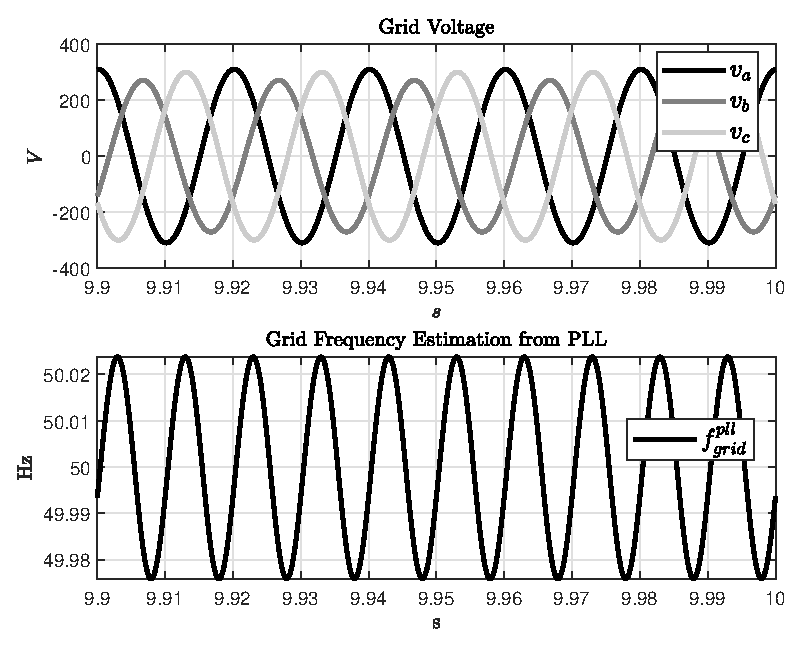
\includegraphics[width = 260pt, angle = 0, 
	keepaspectratio]{figures/sr_without_full_load_1/without_comp_fig_2.eps}
	\captionsetup{width=0.5\textwidth, font=small}	
	\caption{Grid voltage used for the simulation.}
	\label{grid_voltage}
\end{figure}
\begin{figure}[H]
	\centering
	\begin{subfigure}{0.5\textwidth}
		\centering
		\includegraphics[width = 200pt, angle = 0, 
		keepaspectratio]{figures/sr_without_full_load_1/without_comp_fig_4.eps}
		\captionsetup{width=0.65\textwidth, font=footnotesize}	
		\caption{Output current and voltage.}
		\label{}
	\end{subfigure}%
	\begin{subfigure}{0.5\textwidth}
		\centering
		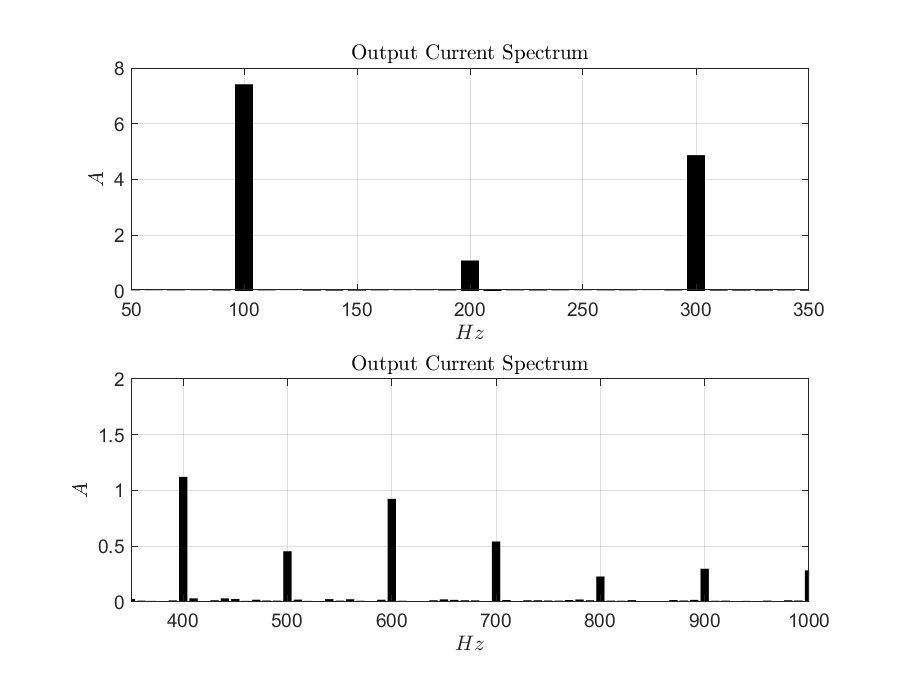
\includegraphics[width = 235pt, angle = 0, 
		keepaspectratio]{figures/sr_without_full_load_1/output_current_spectrum.eps}
		\captionsetup{width=0.65\textwidth, font=footnotesize}	
		\caption{Spectrum of the output current.}
		\label{}
	\end{subfigure}
	\captionsetup{width=0.5\textwidth, font=small}	
	\caption{Simulation results - case study 1.}
	\label{}
\end{figure}
\begin{figure}[H]
	\centering
	\begin{subfigure}{0.5\textwidth}
		\centering
		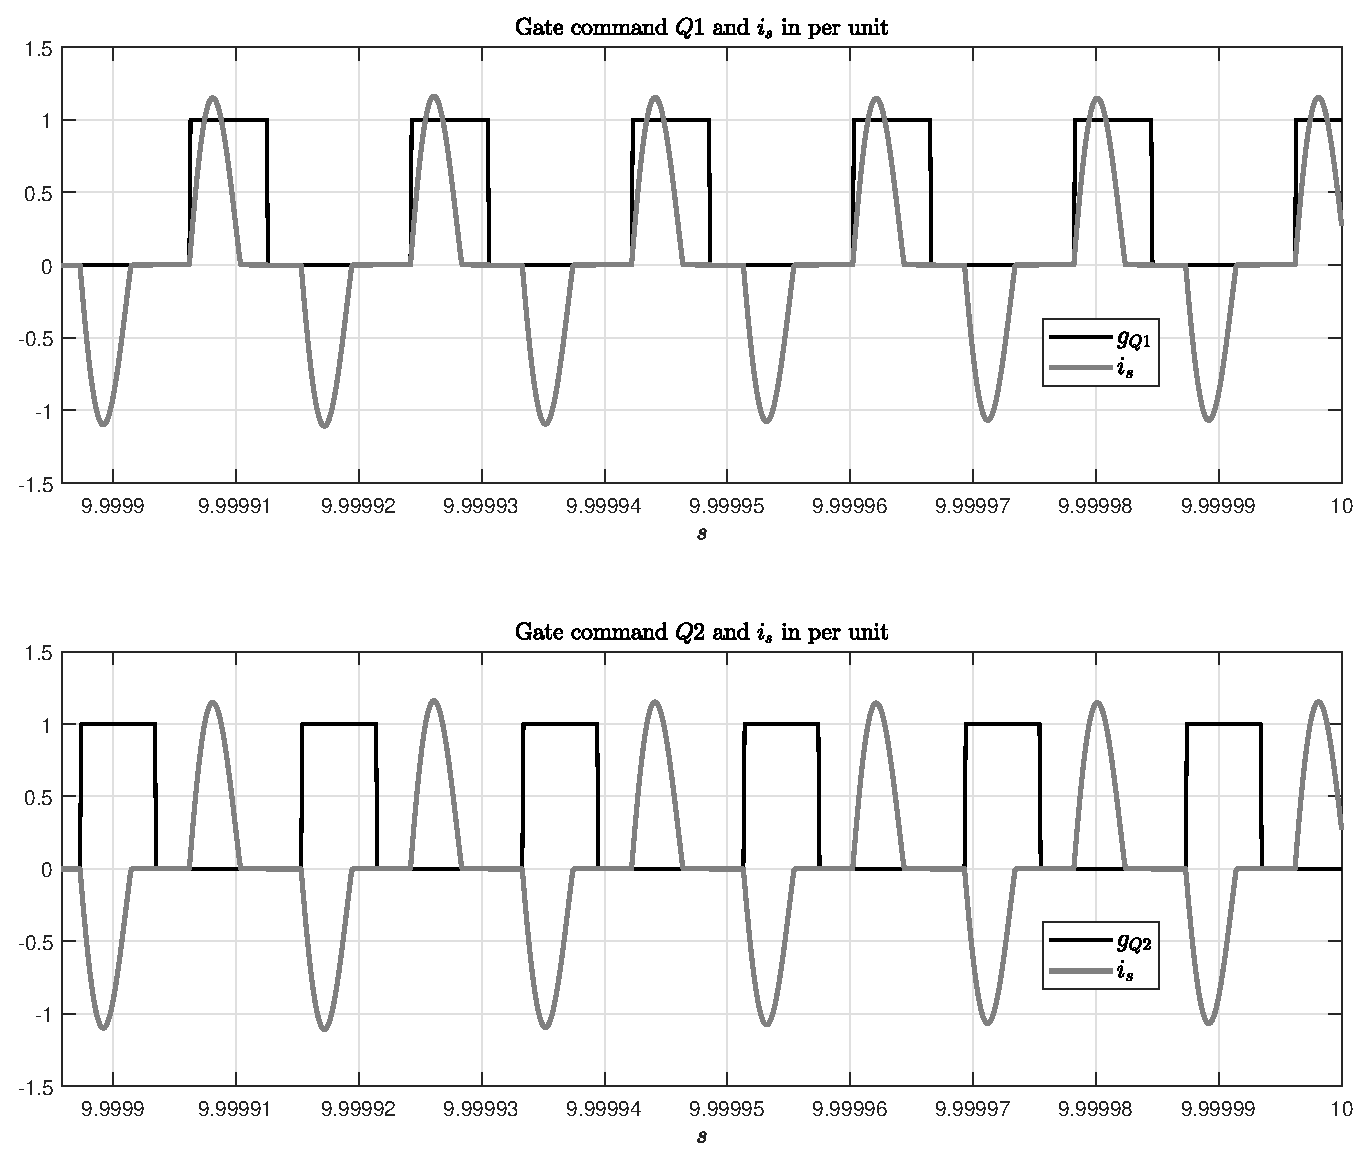
\includegraphics[width = 215pt, angle = 0, 
		keepaspectratio]{figures/sr_without_full_load_1/without_comp_fig_1.eps}
		\captionsetup{width=0.65\textwidth, font=footnotesize}	
		\caption{Switch firing command and $i_s(t)$ resonance current.}
		\label{}
	\end{subfigure}%
	\begin{subfigure}{0.5\textwidth}
		\centering
		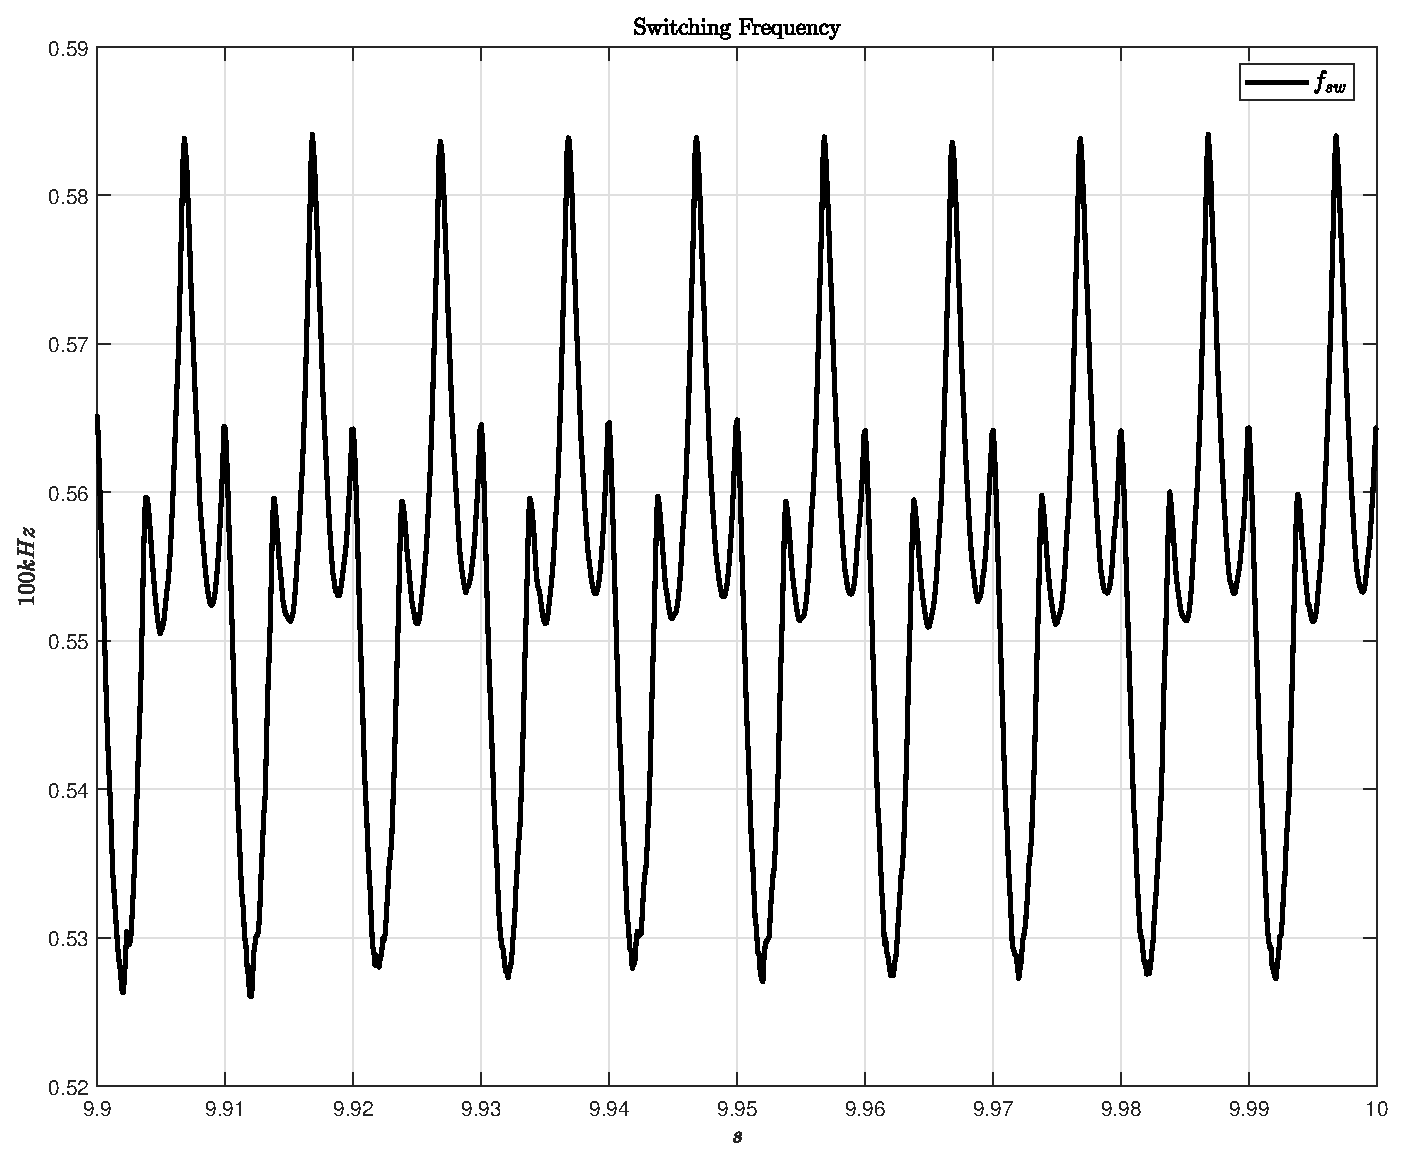
\includegraphics[width = 215pt, angle = 0, 
		keepaspectratio]{figures/sr_without_full_load_1/without_comp_fig_5.eps}
		\captionsetup{width=0.65\textwidth, font=footnotesize}	
		\caption{Control output (frequency switching).}
		\label{}
	\end{subfigure}
	\captionsetup{width=0.5\textwidth, font=small}	
	\caption{Simulation results - case study 1.}
	\label{}
\end{figure}

\section{Case study 2}
For this second case study the following settings are considered:
\begin{itemize}
	\item[--] Harmonic compensator enabled;
	\item[--] $i_{out}^{ref}=\SI{100}{\ampere}$;
	\item[--] $R_{load}=\SI{0.1}{\ohm}$;	
	\item[--] $L_{load}=\SI{25}{\micro\henry}$.
\end{itemize}
\begin{figure}[H]
	\centering
	\includegraphics[width = 260pt, angle = 0, 
	keepaspectratio]{figures/sr_with_full_load_1/with_comp_fig_2.eps}
	\captionsetup{width=0.5\textwidth, font=small}	
	\caption{Grid voltage used for the simulation.}
	\label{}
\end{figure}
\begin{figure}[H]
	\centering
	\begin{subfigure}{0.5\textwidth}
		\centering
		\includegraphics[width = 200pt, angle = 0, 
		keepaspectratio]{figures/sr_with_full_load_1/with_comp_fig_4.eps}
		\captionsetup{width=0.65\textwidth, font=footnotesize}	
		\caption{Output current and voltage.}
		\label{}
	\end{subfigure}%
	\begin{subfigure}{0.5\textwidth}
		\centering
		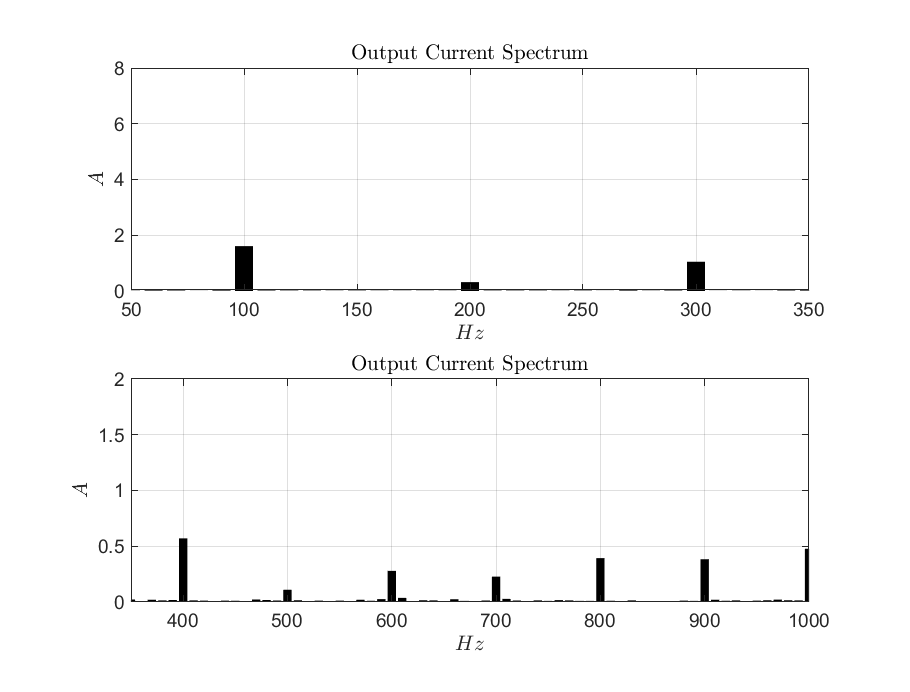
\includegraphics[width = 235pt, angle = 0, 
		keepaspectratio]{figures/sr_with_full_load_1/output_current_spectrum.eps}
		\captionsetup{width=0.65\textwidth, font=footnotesize}	
		\caption{Spectrum of the output current.}
		\label{}
	\end{subfigure}
	\captionsetup{width=0.5\textwidth, font=small}	
	\caption{Simulation results - case study 2.}
	\label{}
\end{figure}
\begin{figure}[H]
	\centering
	\begin{subfigure}{0.5\textwidth}
		\centering
		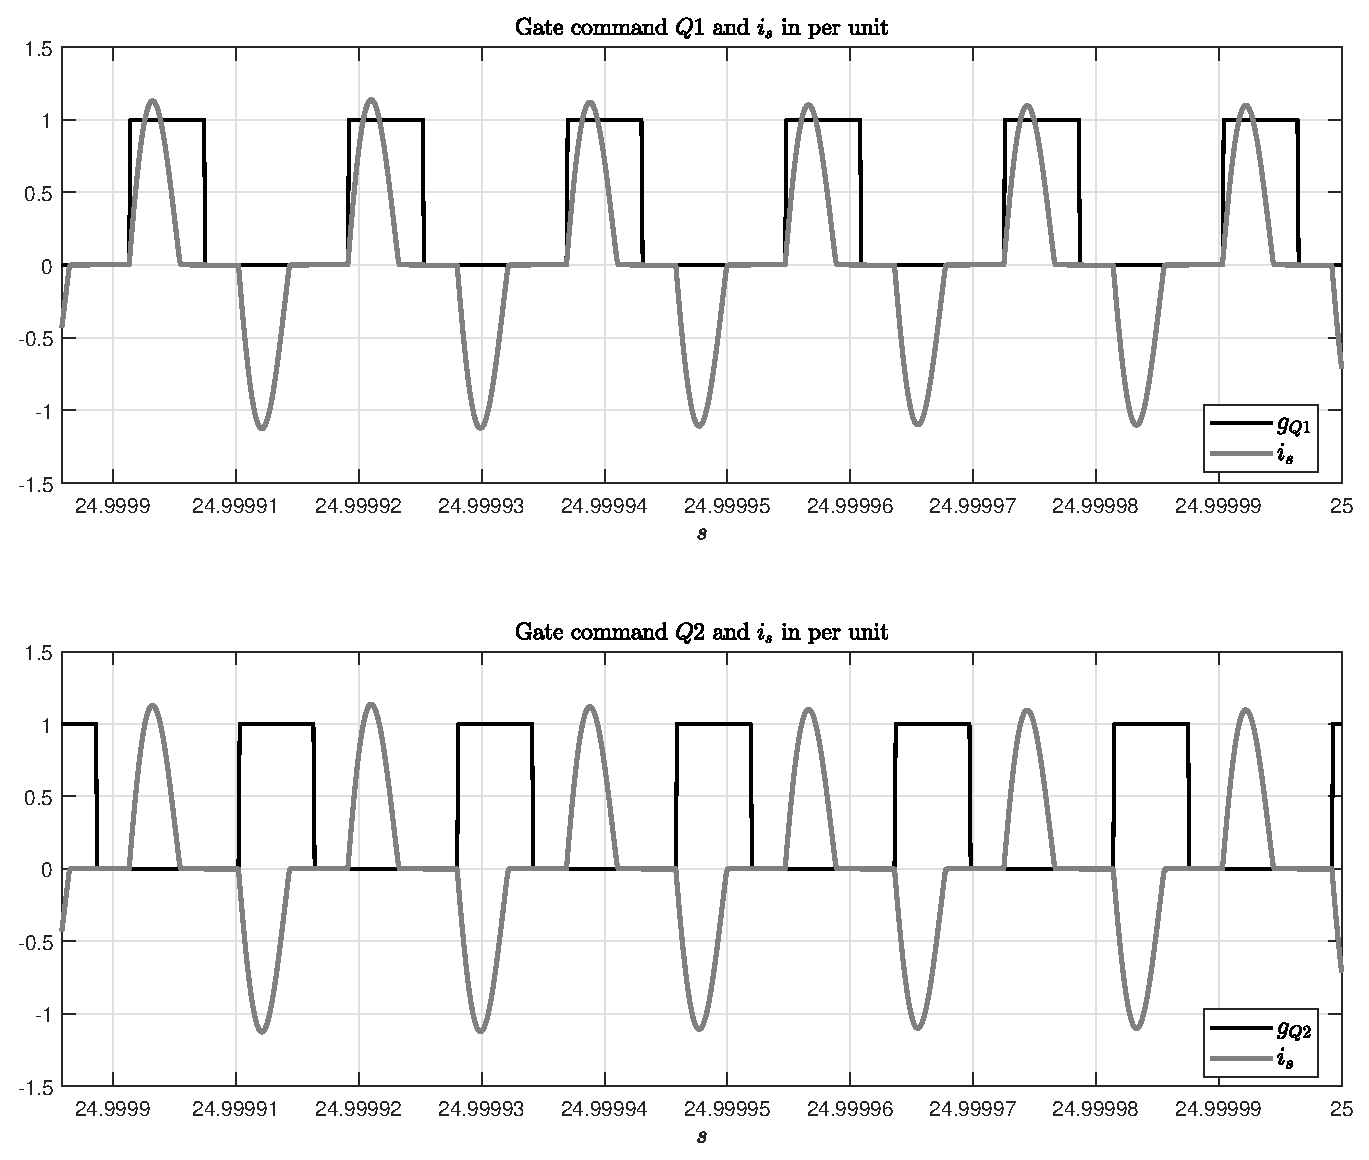
\includegraphics[width = 215pt, angle = 0, 
		keepaspectratio]{figures/sr_with_full_load_1/with_comp_fig_1.eps}
		\captionsetup{width=0.65\textwidth, font=footnotesize}	
		\caption{Switch firing command and $i_s(t)$ resonance current.}
		\label{}
	\end{subfigure}%
	\begin{subfigure}{0.5\textwidth}
		\centering
		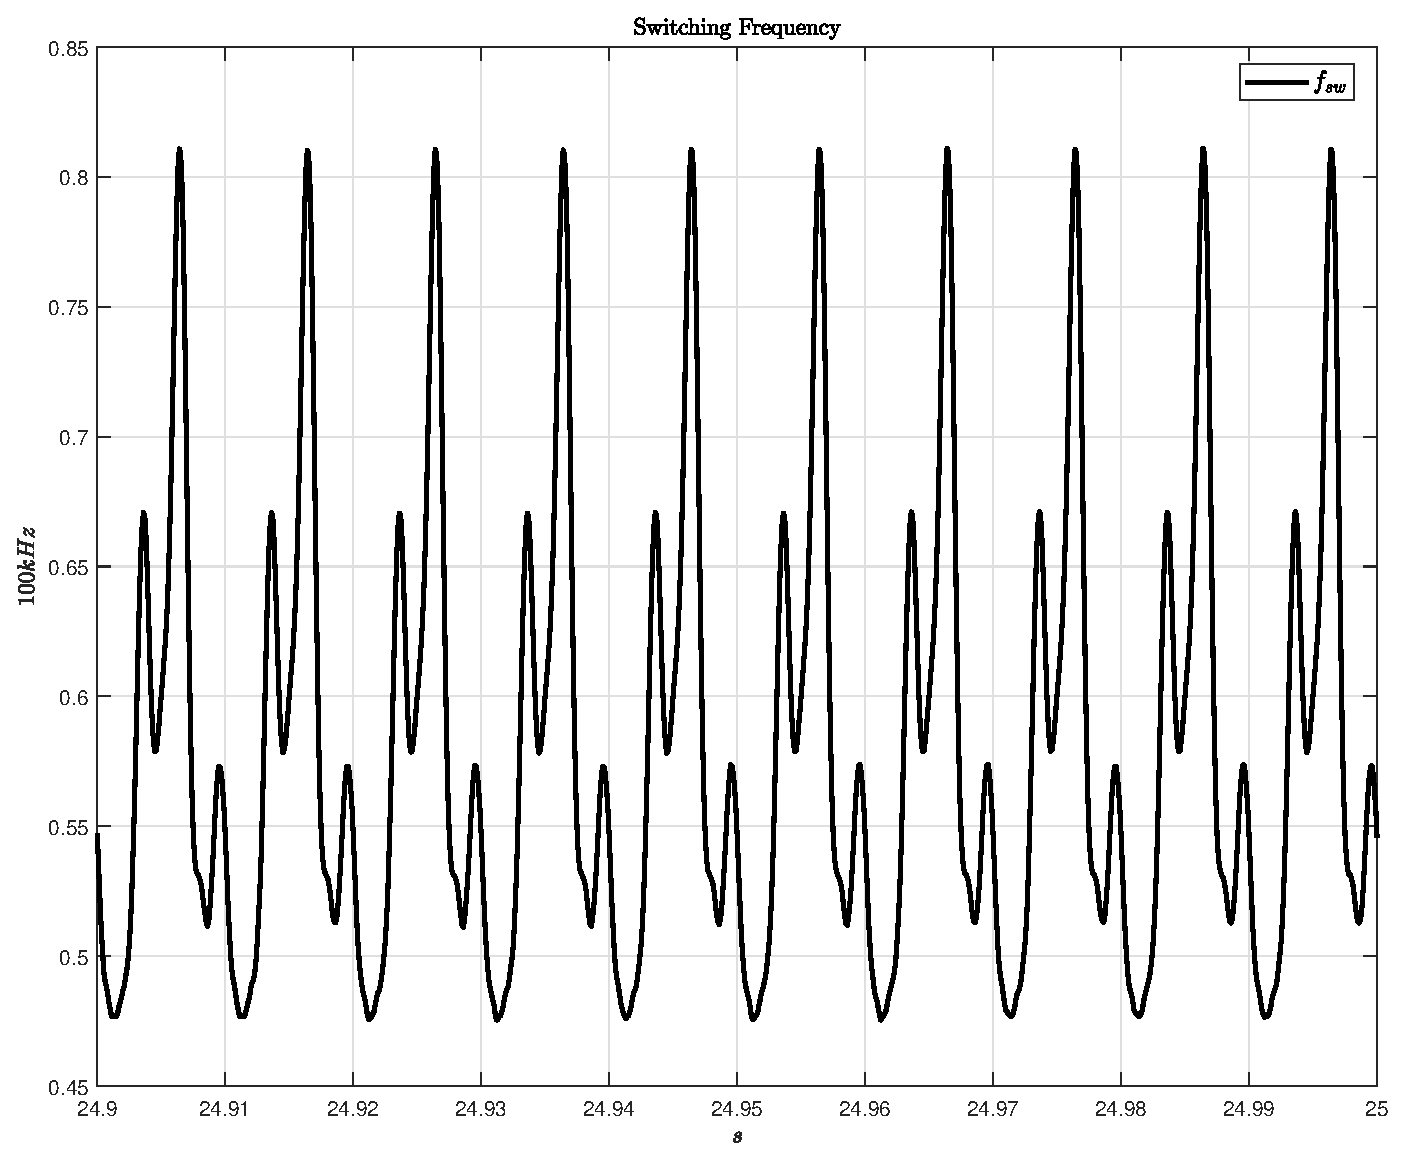
\includegraphics[width = 215pt, angle = 0, 
		keepaspectratio]{figures/sr_with_full_load_1/with_comp_fig_5.eps}
		\captionsetup{width=0.65\textwidth, font=footnotesize}	
		\caption{Control output (frequency switching).}
		\label{}
	\end{subfigure}
	\captionsetup{width=0.5\textwidth, font=small}	
	\caption{Simulation results - case study 2.}
	\label{}
\end{figure}

\section{Case study 3}
For the third case study the following settings are considered:
\begin{itemize}
	\item[--] Harmonic compensator is disabled;
	\item[--] $i_{out}^{ref}=\SI{100}{\ampere}$;
	\item[--] $R_{load}=\SI{0.1}{\ohm}$;	
	\item[--] $L_{load}=\SI{250}{\micro\henry}$.
\end{itemize}
\begin{figure}[H]
	\centering
	\includegraphics[width = 260pt, angle = 0, 
	keepaspectratio]{figures/sr_without_full_load_2/without_comp_fig_2.eps}
	\captionsetup{width=0.5\textwidth, font=small}	
	\caption{Grid voltage used for the simulation.}
	\label{}
\end{figure}
\begin{figure}[H]
	\centering
	\begin{subfigure}{0.5\textwidth}
		\centering
		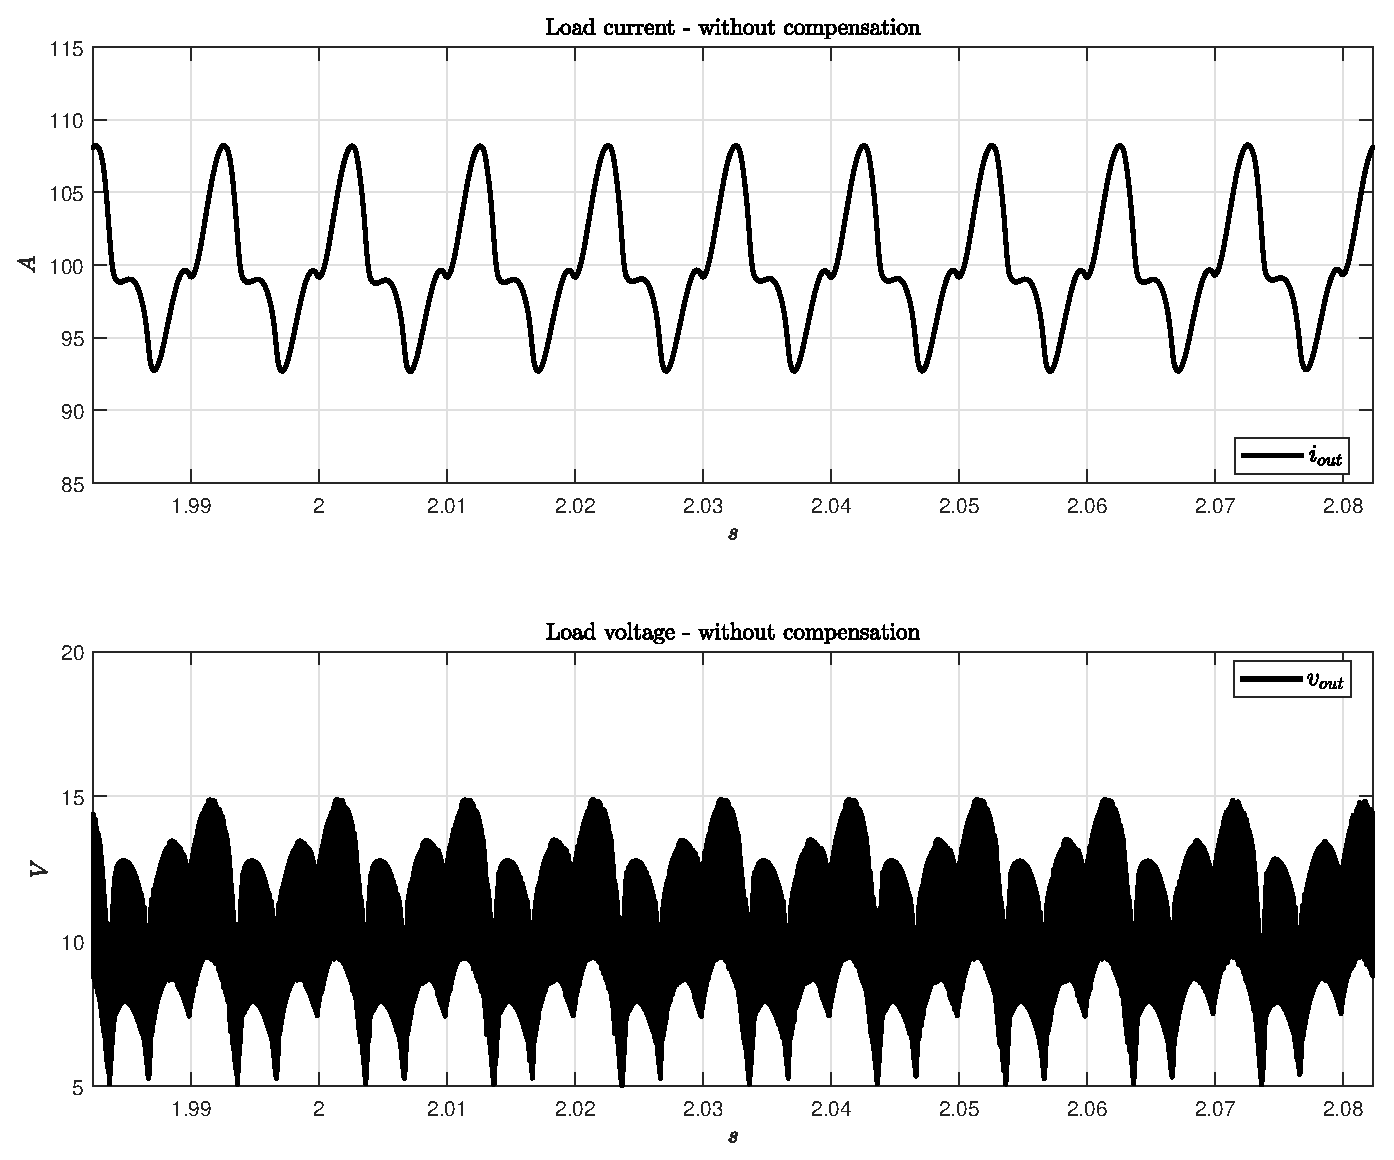
\includegraphics[width = 200pt, angle = 0, 
		keepaspectratio]{figures/sr_without_full_load_2/without_comp_fig_4.eps}
		\captionsetup{width=0.65\textwidth, font=footnotesize}	
		\caption{Output current and voltage.}
		\label{}
	\end{subfigure}%
	\begin{subfigure}{0.5\textwidth}
		\centering
		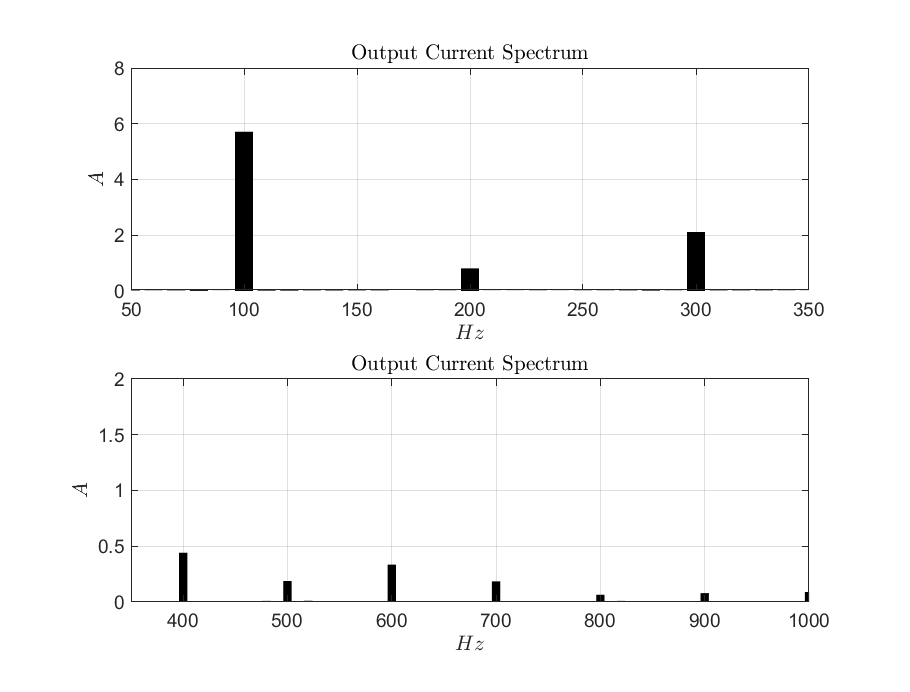
\includegraphics[width = 235pt, angle = 0, 
		keepaspectratio]{figures/sr_without_full_load_2/output_current_spectrum.eps}
		\captionsetup{width=0.65\textwidth, font=footnotesize}	
		\caption{Spectrum of the output current.}
		\label{}
	\end{subfigure}
	\captionsetup{width=0.5\textwidth, font=small}	
	\caption{Simulation results - case study 3.}
	\label{}
\end{figure}
\begin{figure}[H]
	\centering
	\begin{subfigure}{0.5\textwidth}
		\centering
		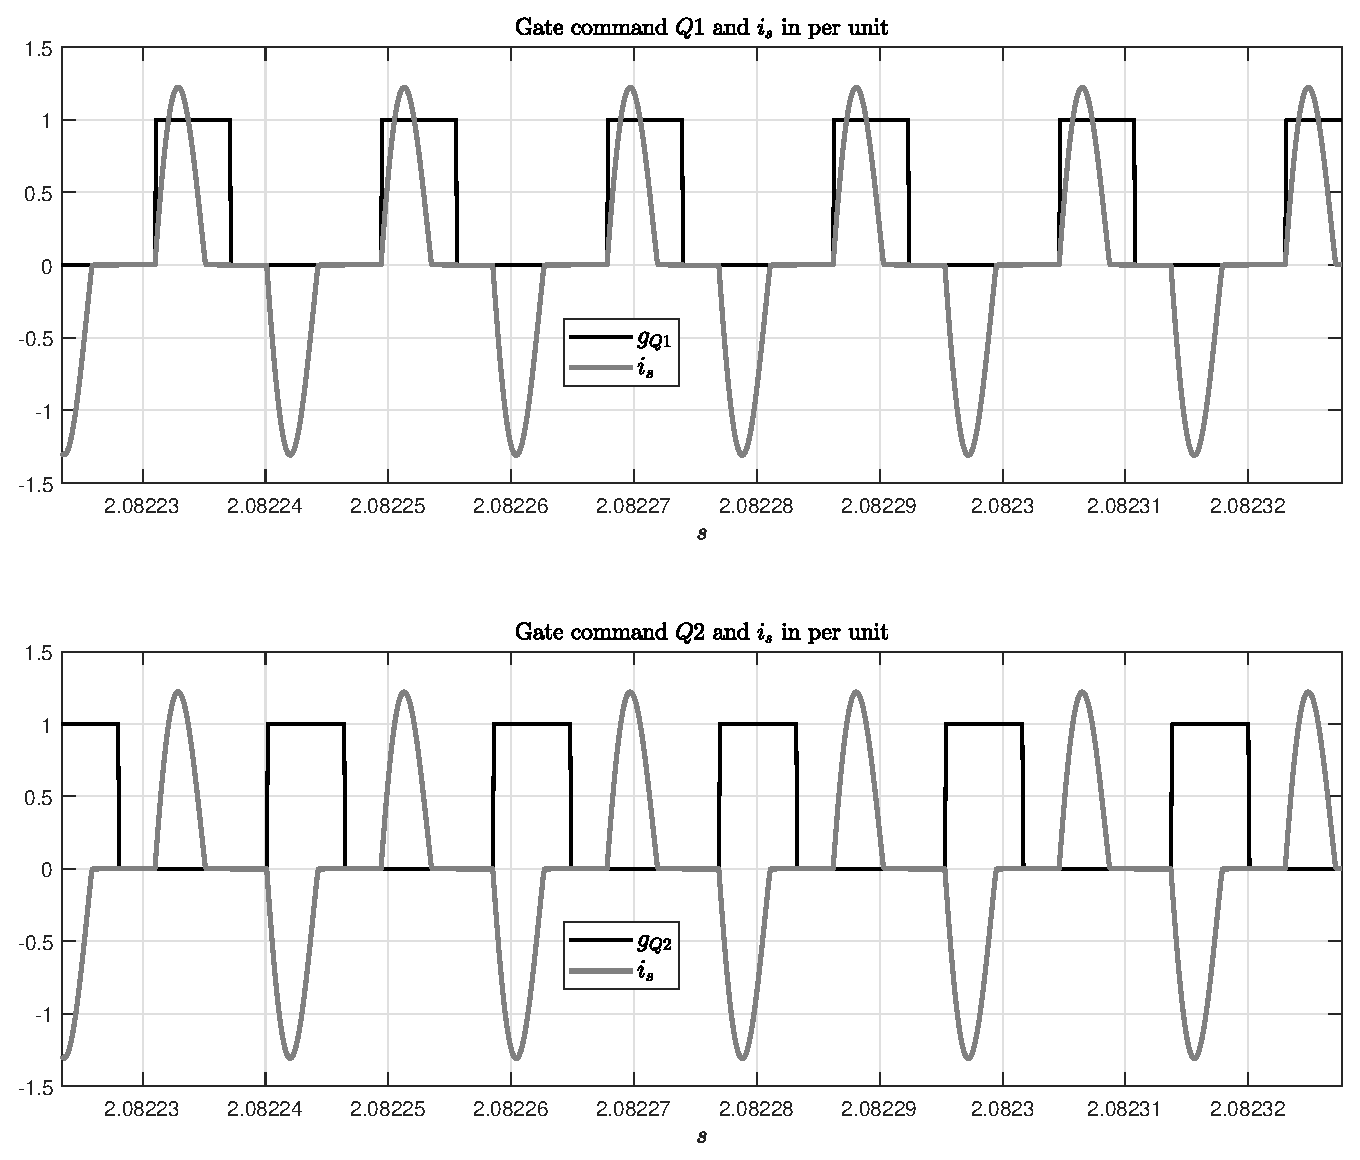
\includegraphics[width = 215pt, angle = 0, 
		keepaspectratio]{figures/sr_without_full_load_2/without_comp_fig_1.eps}
		\captionsetup{width=0.65\textwidth, font=footnotesize}	
		\caption{Switch firing command and $i_s(t)$ resonance current.}
		\label{}
	\end{subfigure}%
	\begin{subfigure}{0.5\textwidth}
		\centering
		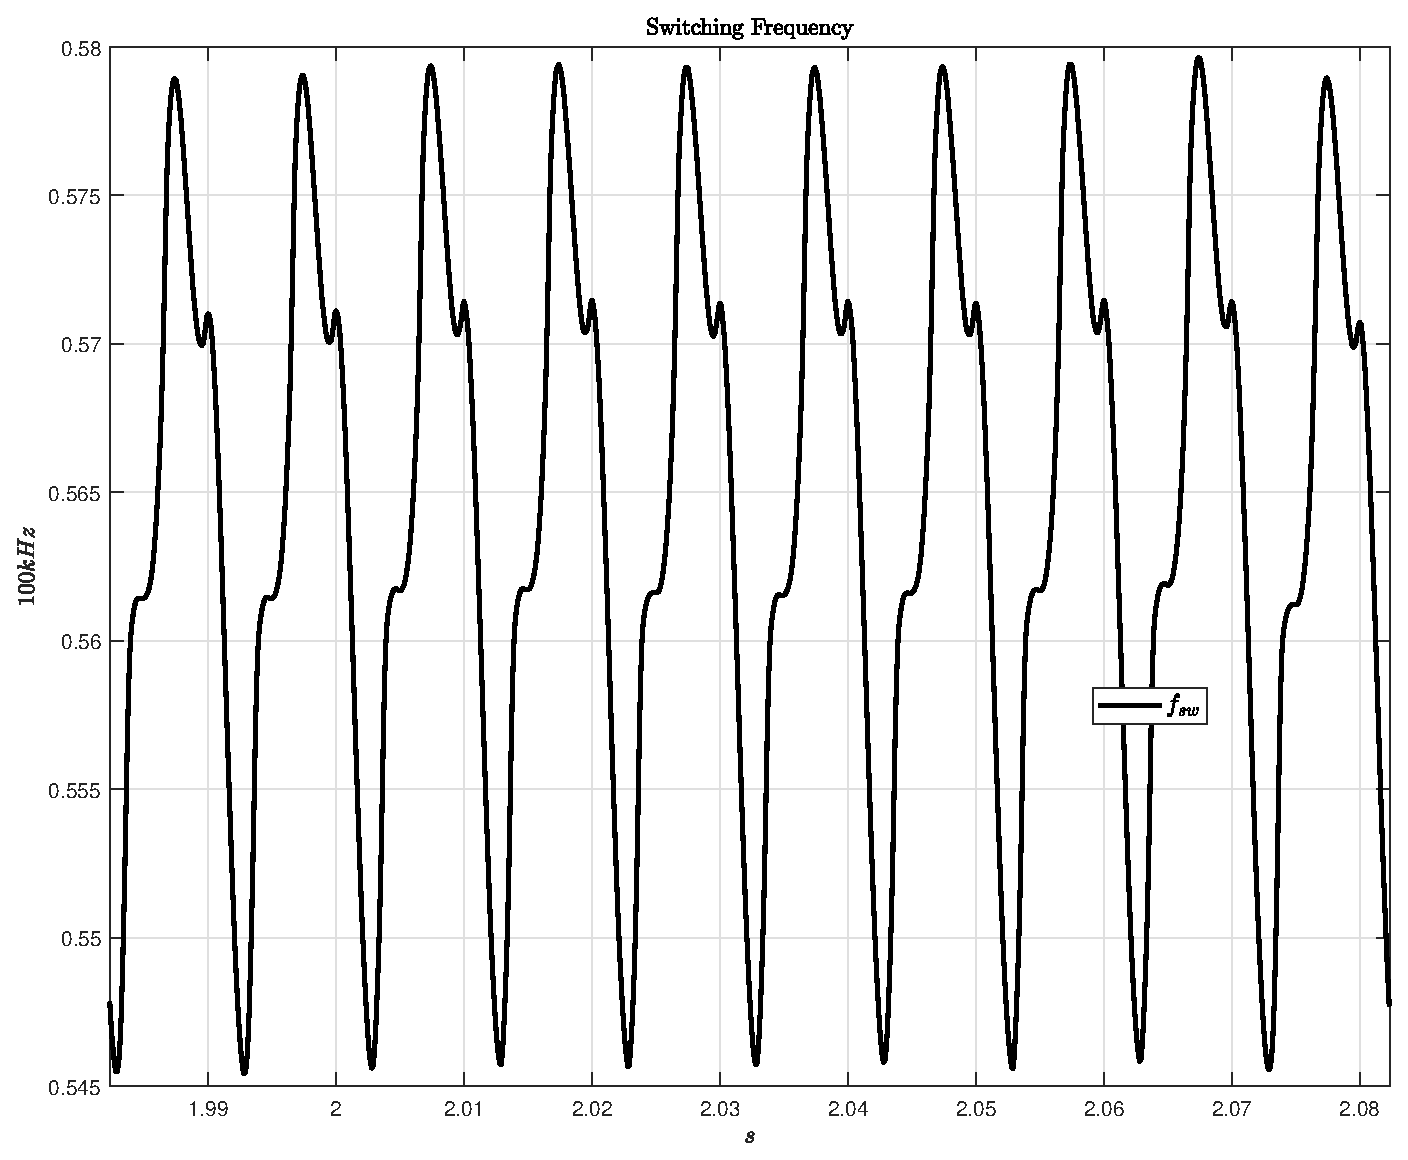
\includegraphics[width = 215pt, angle = 0, 
		keepaspectratio]{figures/sr_without_full_load_2/without_comp_fig_5.eps}
		\captionsetup{width=0.65\textwidth, font=footnotesize}	
		\caption{Control output (frequency switching).}
		\label{}
	\end{subfigure}
	\captionsetup{width=0.5\textwidth, font=small}	
	\caption{Simulation results - case study 3.}
	\label{}
\end{figure}

\section{Case study 4}
For this fourth case study the following settings are considered:
\begin{itemize}
	\item[--] Harmonic compensator enabled;
	\item[--] $i_{out}^{ref}=\SI{100}{\ampere}$;
	\item[--] $R_{load}=\SI{0.1}{\ohm}$;	
	\item[--] $L_{load}=\SI{250}{\micro\henry}$.
\end{itemize}
\begin{figure}[H]
	\centering
	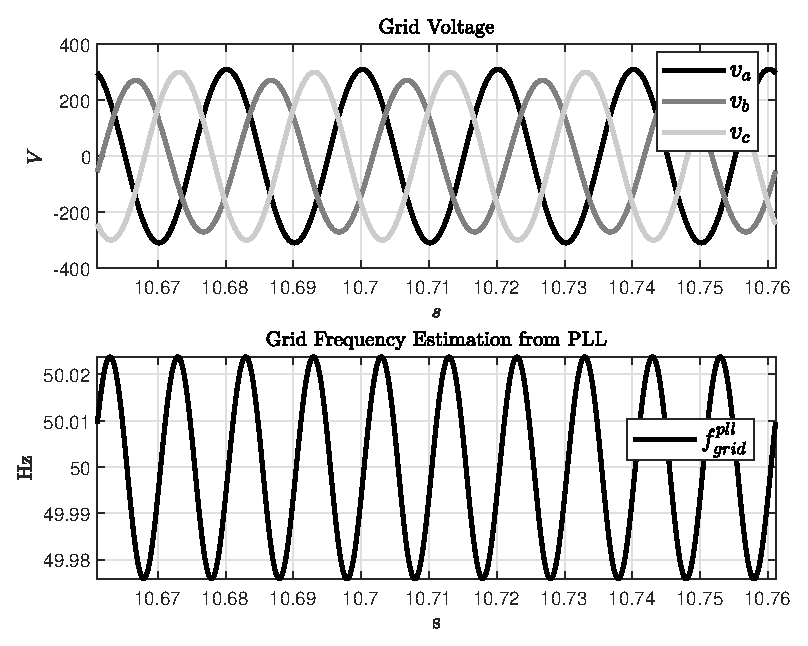
\includegraphics[width = 260pt, angle = 0, 
	keepaspectratio]{figures/sr_with_full_load_2/with_comp_fig_2.eps}
	\captionsetup{width=0.5\textwidth, font=small}	
	\caption{Grid voltage used for the simulation.}
	\label{}
\end{figure}
\begin{figure}[H]
	\centering
	\begin{subfigure}{0.5\textwidth}
		\centering
		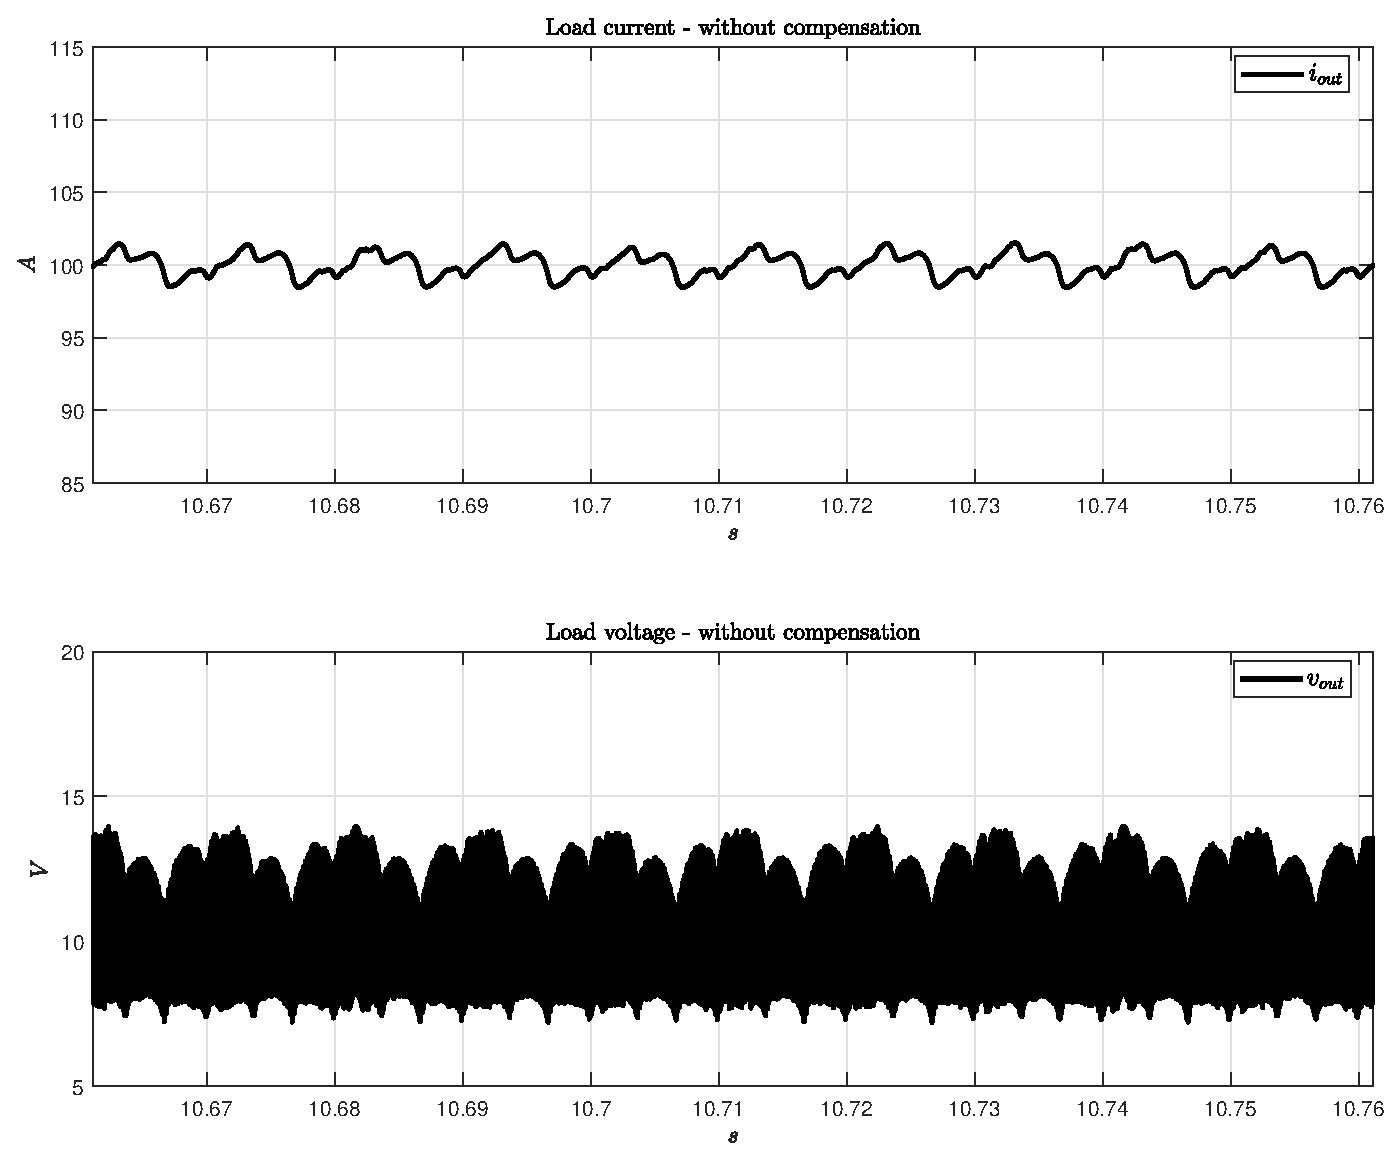
\includegraphics[width = 200pt, angle = 0, 
		keepaspectratio]{figures/sr_with_full_load_2/with_comp_fig_4.eps}
		\captionsetup{width=0.65\textwidth, font=footnotesize}	
		\caption{Output current and voltage.}
		\label{}
	\end{subfigure}%
	\begin{subfigure}{0.5\textwidth}
		\centering
		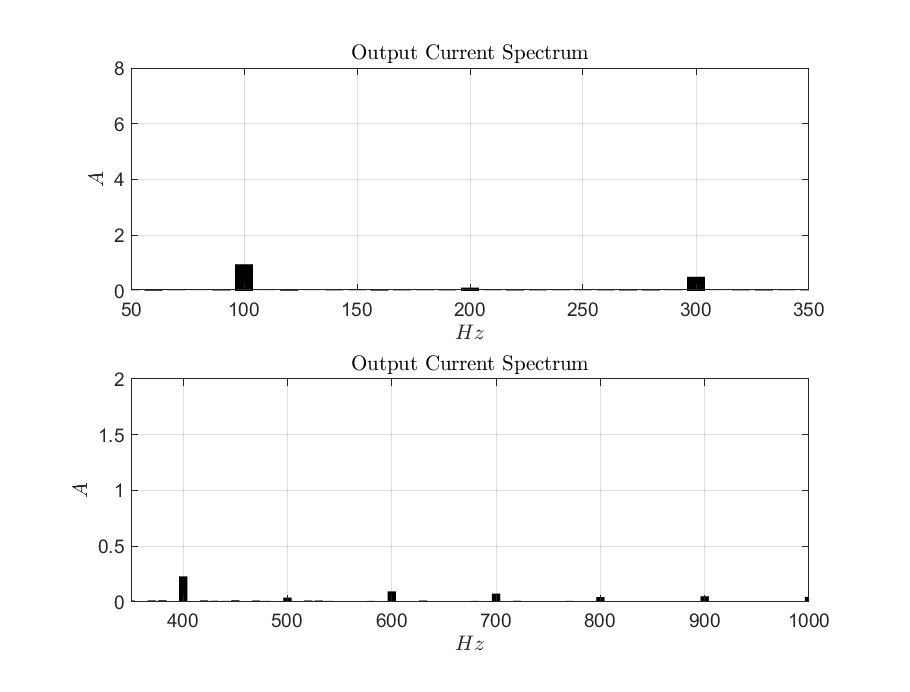
\includegraphics[width = 235pt, angle = 0, 
		keepaspectratio]{figures/sr_with_full_load_2/output_current_spectrum.eps}
		\captionsetup{width=0.65\textwidth, font=footnotesize}	
		\caption{Spectrum of the output current.}
		\label{}
	\end{subfigure}
	\captionsetup{width=0.5\textwidth, font=small}	
	\caption{Simulation results - case study 4.}
	\label{}
\end{figure}
\begin{figure}[H]
	\centering
	\begin{subfigure}{0.5\textwidth}
		\centering
		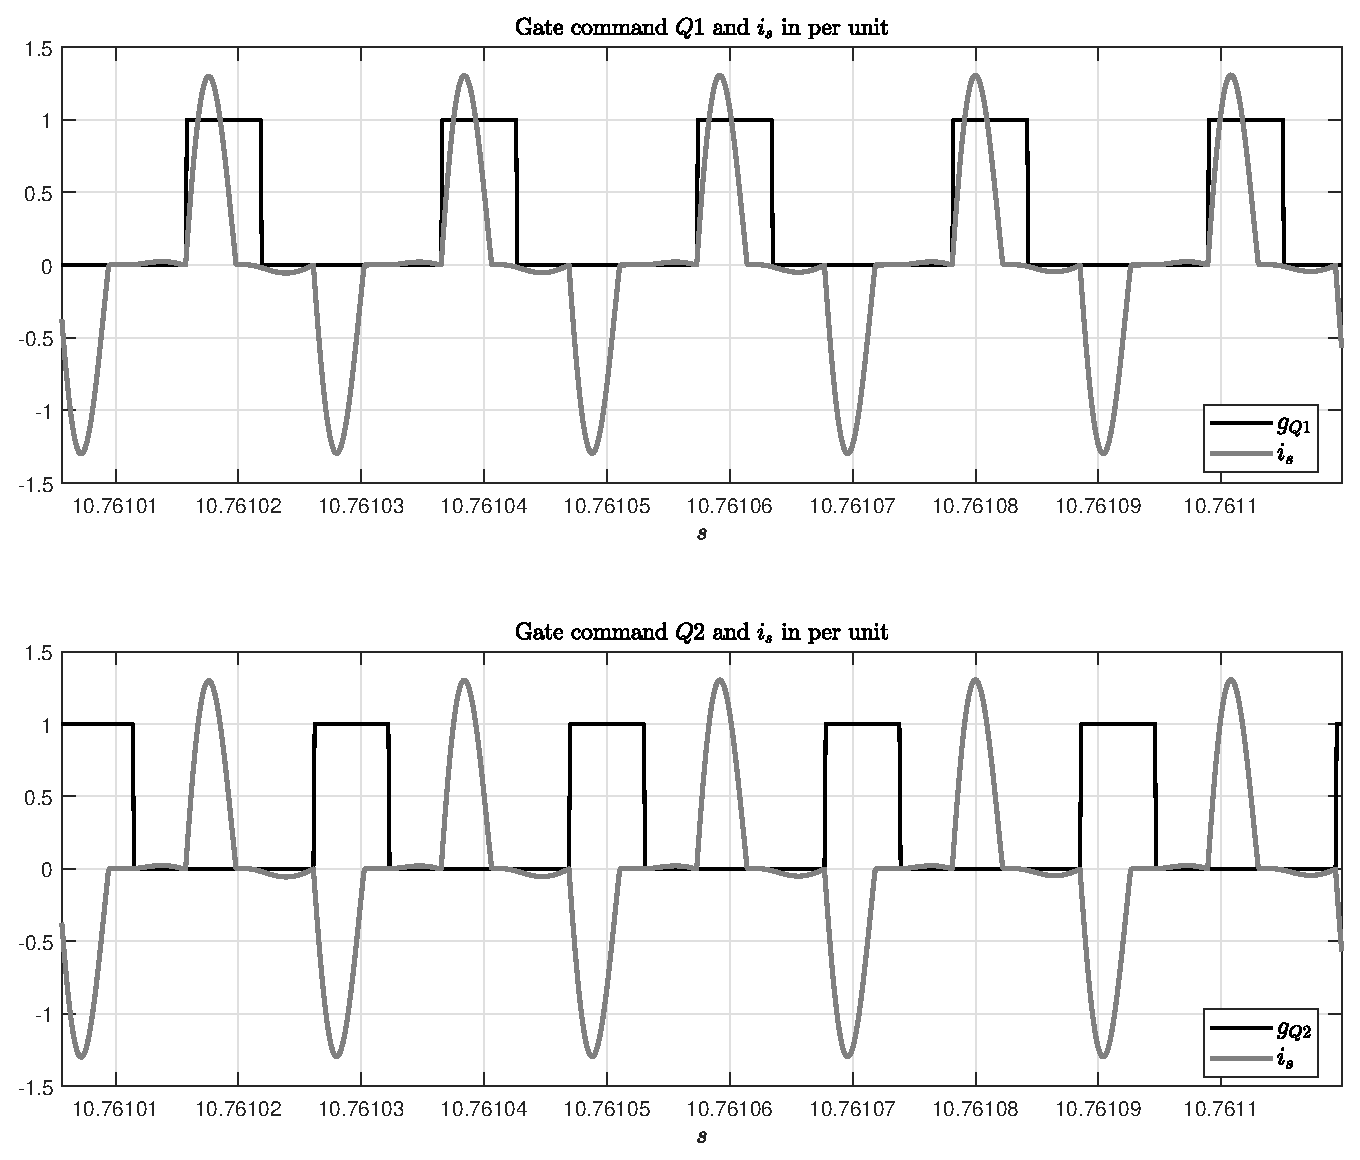
\includegraphics[width = 215pt, angle = 0, 
		keepaspectratio]{figures/sr_with_full_load_2/with_comp_fig_1.eps}
		\captionsetup{width=0.65\textwidth, font=footnotesize}	
		\caption{Switch firing command and $i_s(t)$ resonance current.}
		\label{}
	\end{subfigure}%
	\begin{subfigure}{0.5\textwidth}
		\centering
		\includegraphics[width = 215pt, angle = 0, 
		keepaspectratio]{figures/sr_with_full_load_2/with_comp_fig_5.eps}
		\captionsetup{width=0.65\textwidth, font=footnotesize}	
		\caption{Control output (frequency switching).}
		\label{}
	\end{subfigure}
	\captionsetup{width=0.5\textwidth, font=small}	
	\caption{Simulation results - case study 4.}
	\label{}
\end{figure}

\section{Case study 5}
For the fifth case study the following settings are considered:
\begin{itemize}
	\item[--] Harmonic compensator is disabled;
	\item[--] $i_{out}^{ref}=\SI{5}{\ampere}$;
	\item[--] $R_{load}=\SI{2}{\ohm}$;	
	\item[--] $L_{load}=\SI{25}{\micro\henry}$.
\end{itemize}
\begin{figure}[H]
	\centering
	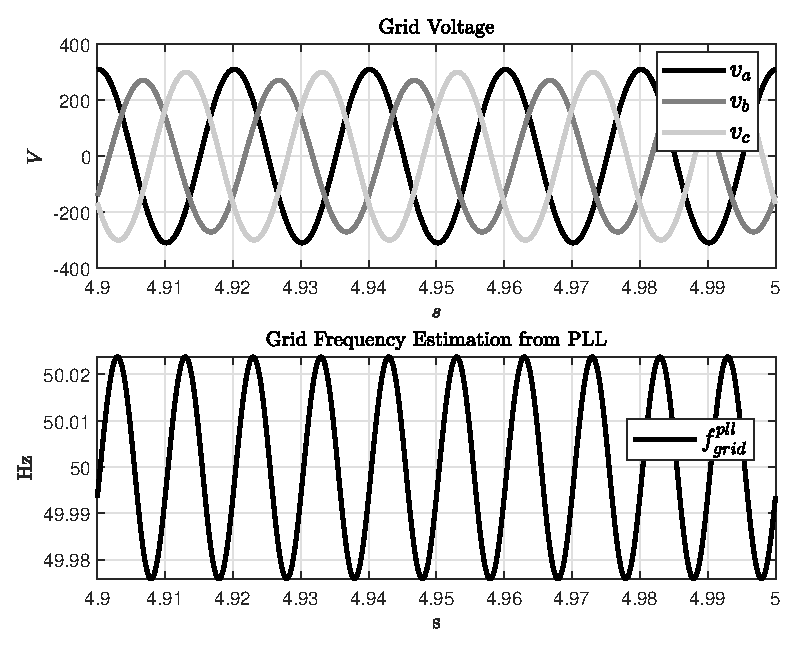
\includegraphics[width = 260pt, angle = 0, 
	keepaspectratio]{figures/sr_without_full_load_3/without_comp_fig_2.eps}
	\captionsetup{width=0.5\textwidth, font=small}	
	\caption{Grid voltage used for the simulation.}
	\label{}
\end{figure}
\begin{figure}[H]
	\centering
	\begin{subfigure}{0.5\textwidth}
		\centering
		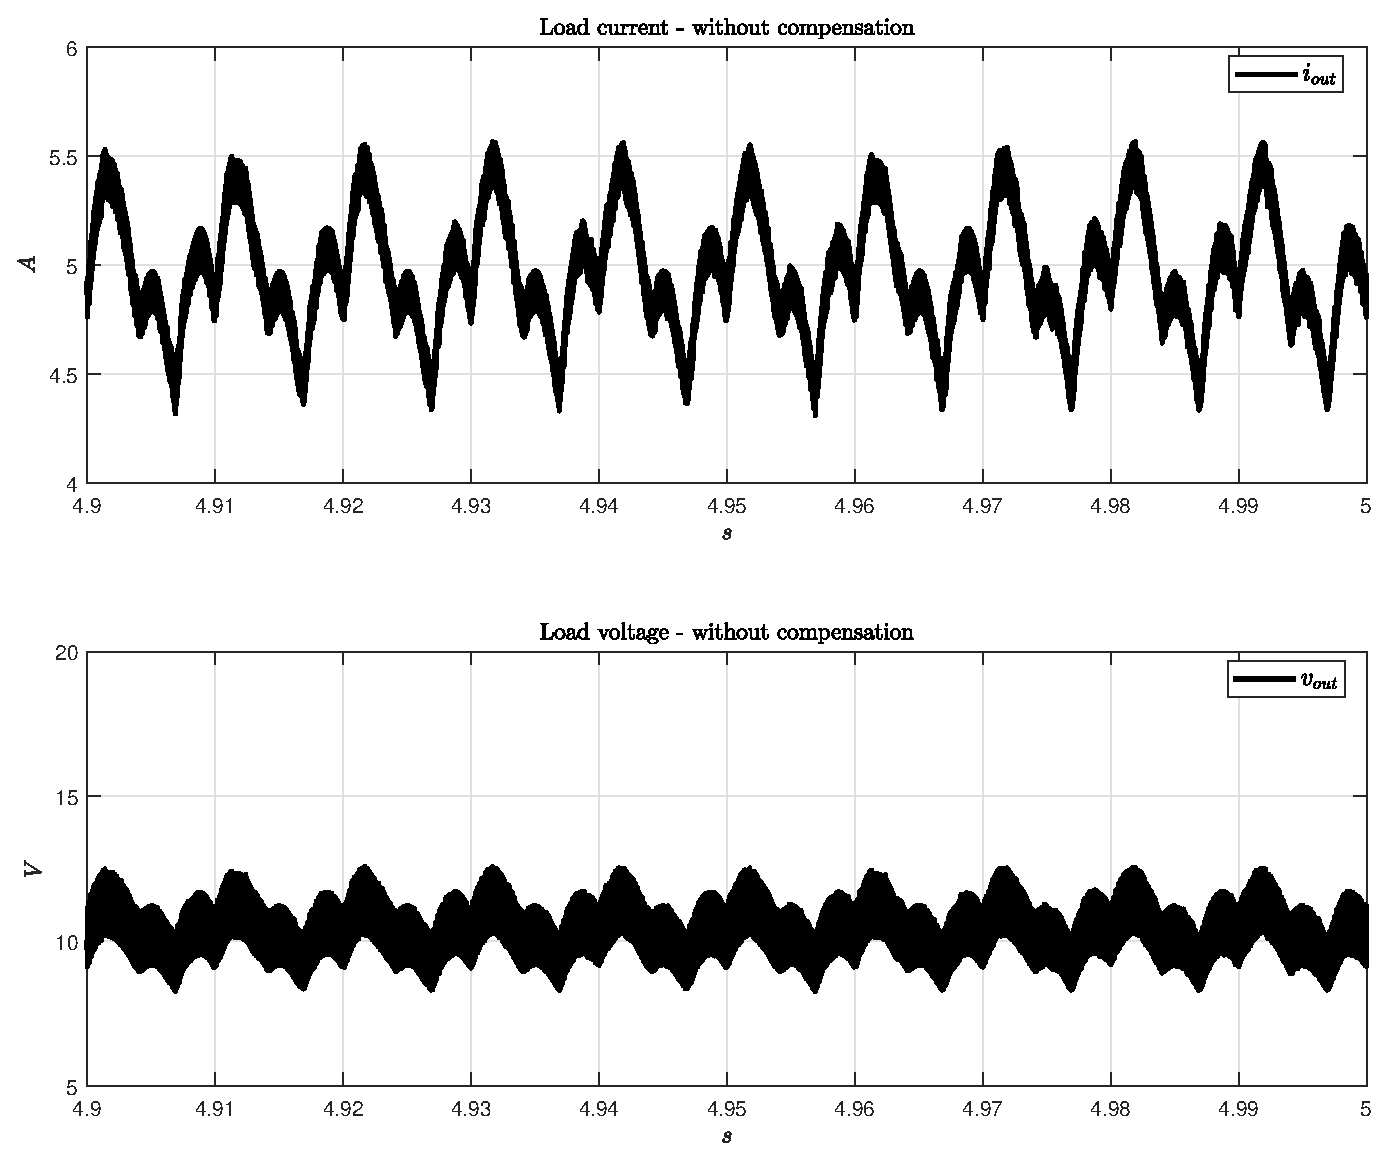
\includegraphics[width = 200pt, angle = 0, 
		keepaspectratio]{figures/sr_without_full_load_3/without_comp_fig_4.eps}
		\captionsetup{width=0.65\textwidth, font=footnotesize}	
		\caption{Output current and voltage.}
		\label{}
	\end{subfigure}%
	\begin{subfigure}{0.5\textwidth}
		\centering
		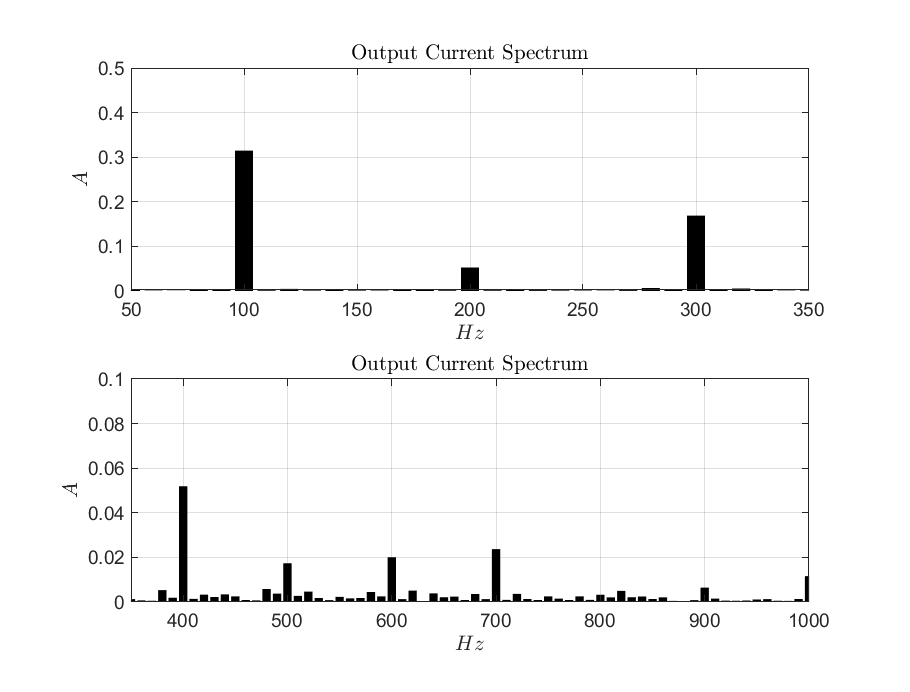
\includegraphics[width = 235pt, angle = 0, 
		keepaspectratio]{figures/sr_without_full_load_3/output_current_spectrum.eps}
		\captionsetup{width=0.65\textwidth, font=footnotesize}	
		\caption{Spectrum of the output current.}
		\label{}
	\end{subfigure}
	\captionsetup{width=0.5\textwidth, font=small}	
	\caption{Simulation results - case study 5.}
	\label{}
\end{figure}
\begin{figure}[H]
	\centering
	\begin{subfigure}{0.5\textwidth}
		\centering
		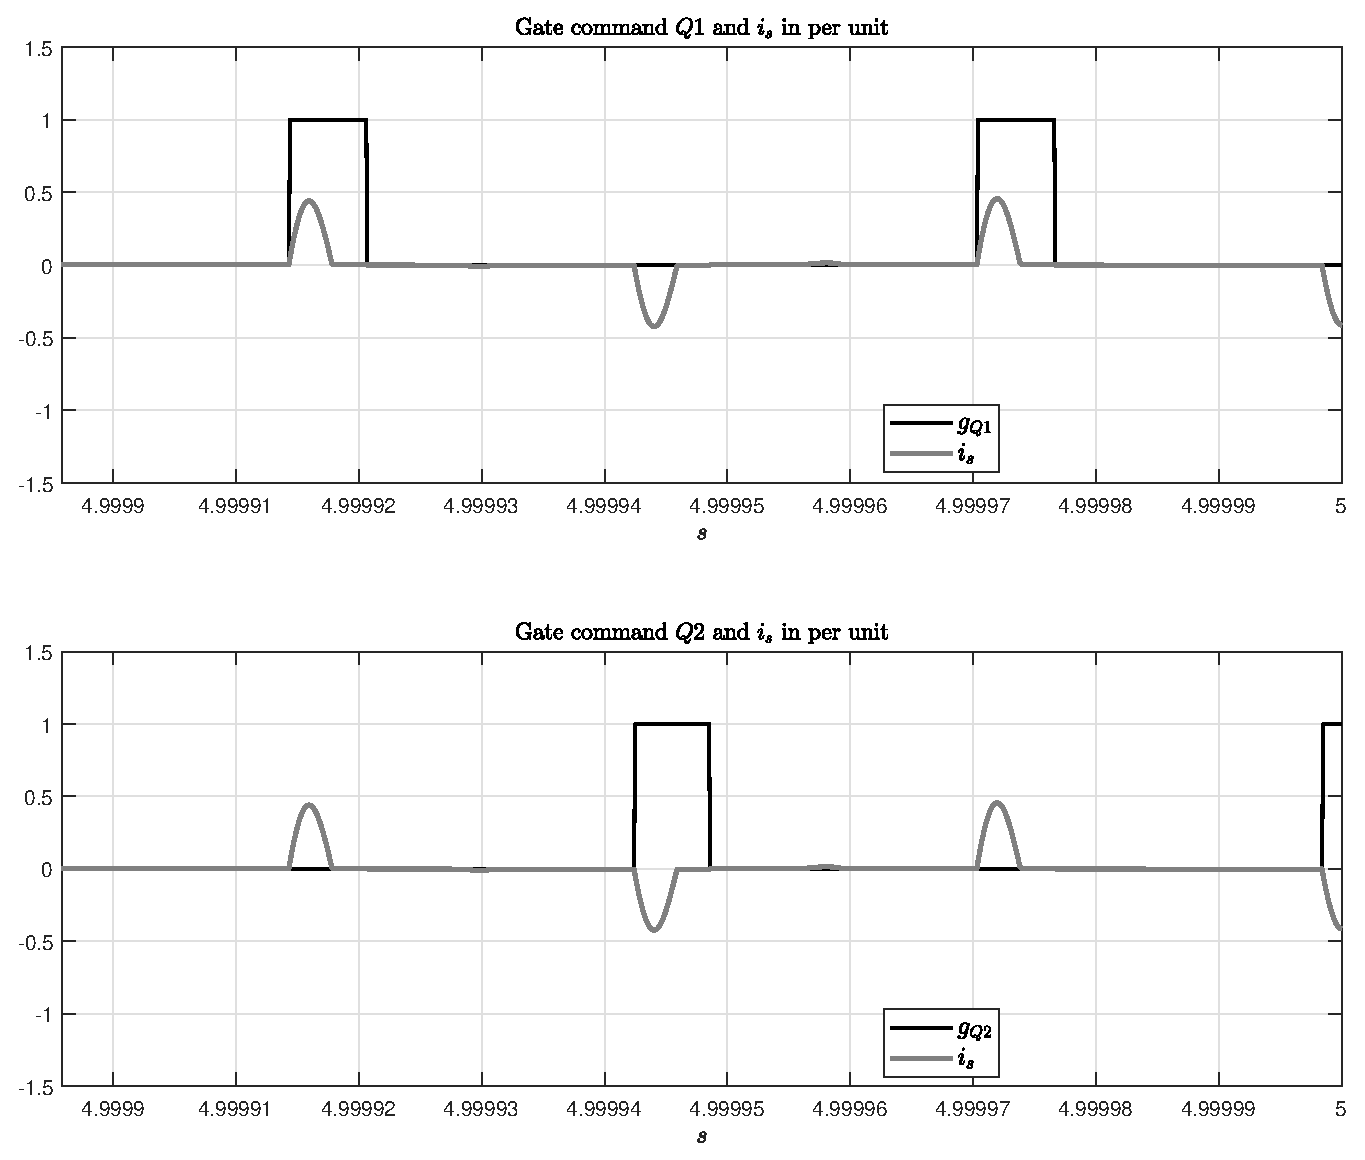
\includegraphics[width = 215pt, angle = 0, 
		keepaspectratio]{figures/sr_without_full_load_3/without_comp_fig_1.eps}
		\captionsetup{width=0.65\textwidth, font=footnotesize}	
		\caption{Switch firing command and $i_s(t)$ resonance current.}
		\label{}
	\end{subfigure}%
	\begin{subfigure}{0.5\textwidth}
		\centering
		\includegraphics[width = 215pt, angle = 0, 
		keepaspectratio]{figures/sr_without_full_load_3/without_comp_fig_5.eps}
		\captionsetup{width=0.65\textwidth, font=footnotesize}	
		\caption{Control output (frequency switching).}
		\label{}
	\end{subfigure}
	\captionsetup{width=0.5\textwidth, font=small}	
	\caption{Simulation results - case study 5.}
	\label{}
\end{figure}

\section{Case study 6}
For this sixth case study the following settings are considered:
\begin{itemize}
	\item[--] Harmonic compensator enabled;
	\item[--] $i_{out}^{ref}=\SI{5}{\ampere}$;
	\item[--] $R_{load}=\SI{2}{\ohm}$;	
	\item[--] $L_{load}=\SI{25}{\micro\henry}$.
\end{itemize}
\begin{figure}[H]
	\centering
	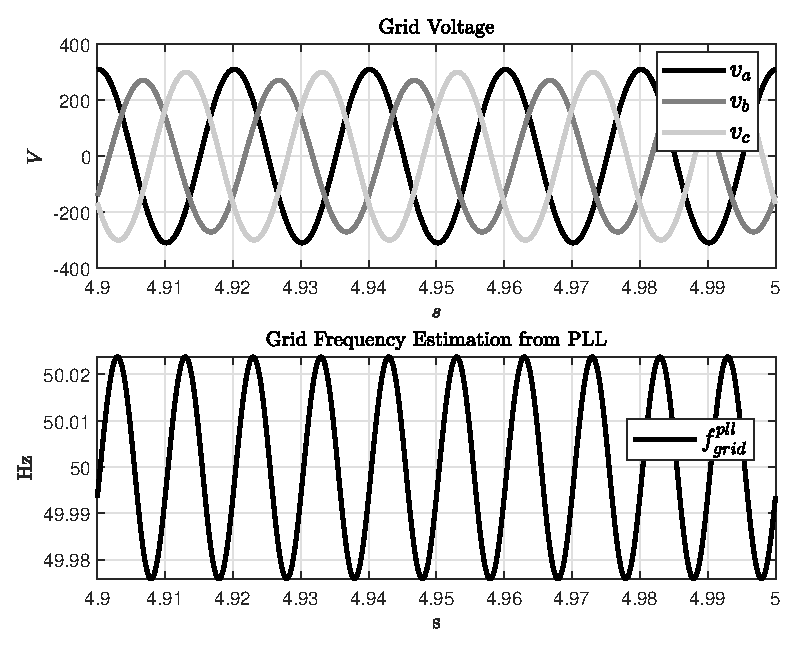
\includegraphics[width = 260pt, angle = 0, 
	keepaspectratio]{figures/sr_with_full_load_3/with_comp_fig_2.eps}
	\captionsetup{width=0.5\textwidth, font=small}	
	\caption{Grid voltage used for the simulation.}
	\label{}
\end{figure}
\begin{figure}[H]
	\centering
	\begin{subfigure}{0.5\textwidth}
		\centering
		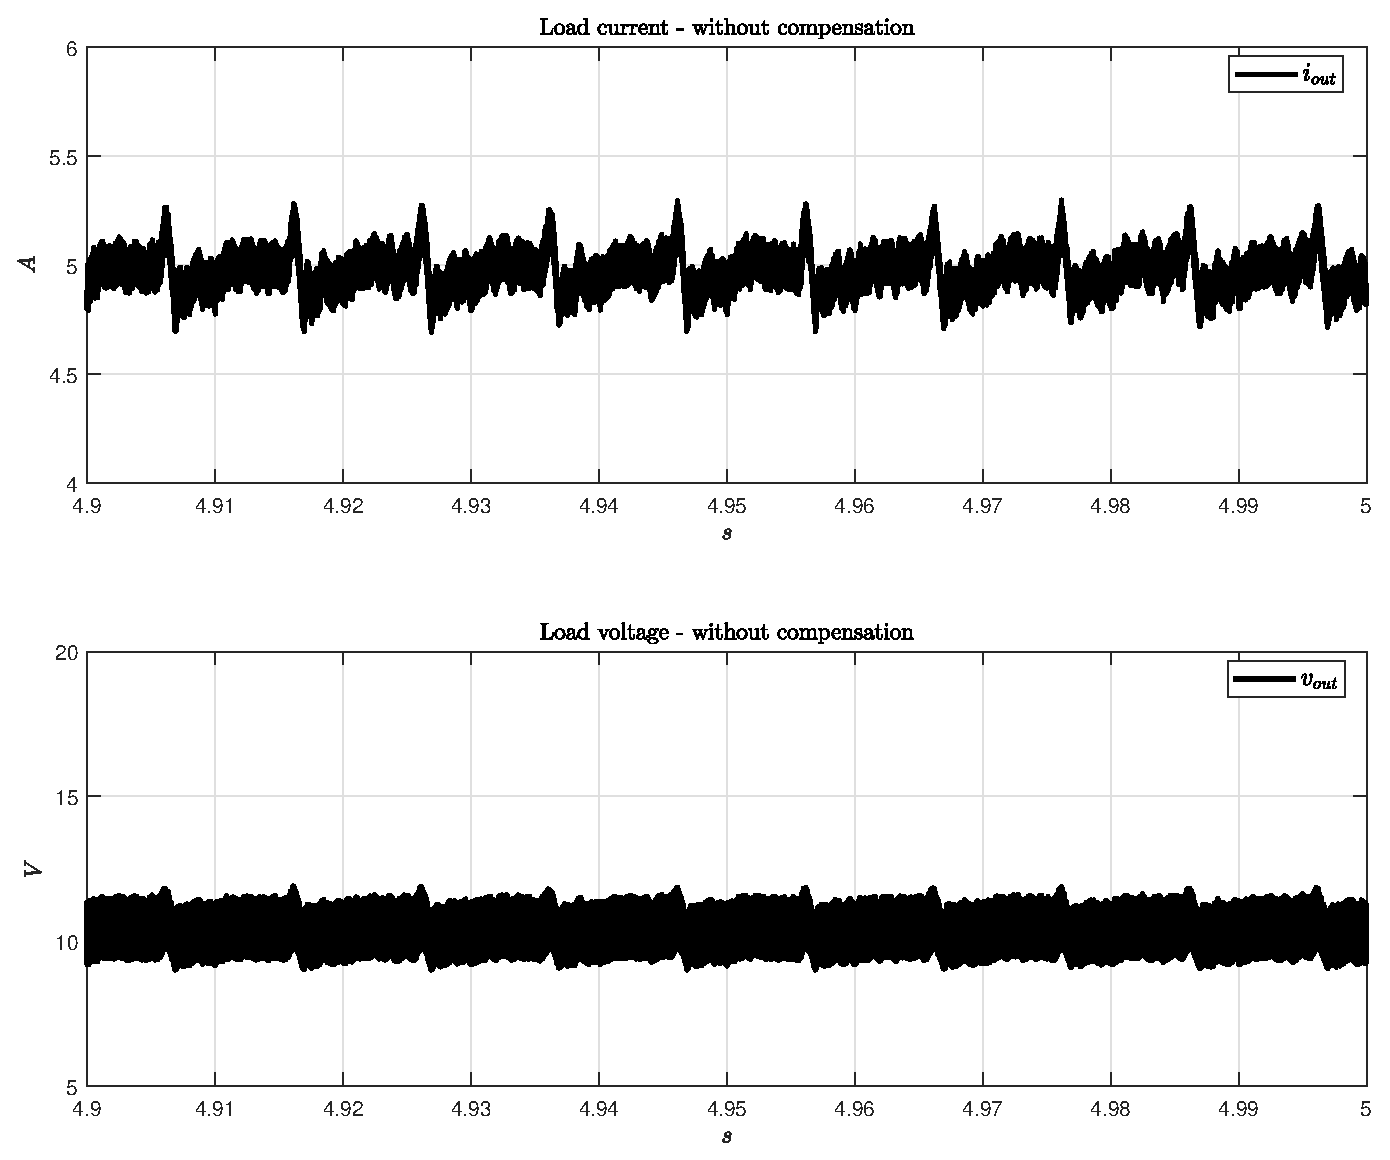
\includegraphics[width = 200pt, angle = 0, 
		keepaspectratio]{figures/sr_with_full_load_3/with_comp_fig_4.eps}
		\captionsetup{width=0.65\textwidth, font=footnotesize}	
		\caption{Output current and voltage.}
		\label{}
	\end{subfigure}%
	\begin{subfigure}{0.5\textwidth}
		\centering
		\includegraphics[width = 235pt, angle = 0, 
		keepaspectratio]{figures/sr_with_full_load_3/output_current_spectrum.eps}
		\captionsetup{width=0.65\textwidth, font=footnotesize}	
		\caption{Spectrum of the output current.}
		\label{}
	\end{subfigure}
	\captionsetup{width=0.5\textwidth, font=small}	
	\caption{Simulation results - case study 6.}
	\label{}
\end{figure}
\begin{figure}[H]
	\centering
	\begin{subfigure}{0.5\textwidth}
		\centering
		\includegraphics[width = 215pt, angle = 0, 
		keepaspectratio]{figures/sr_with_full_load_3/with_comp_fig_1.eps}
		\captionsetup{width=0.65\textwidth, font=footnotesize}	
		\caption{Switch firing command and $i_s(t)$ resonance current.}
		\label{}
	\end{subfigure}%
	\begin{subfigure}{0.5\textwidth}
		\centering
		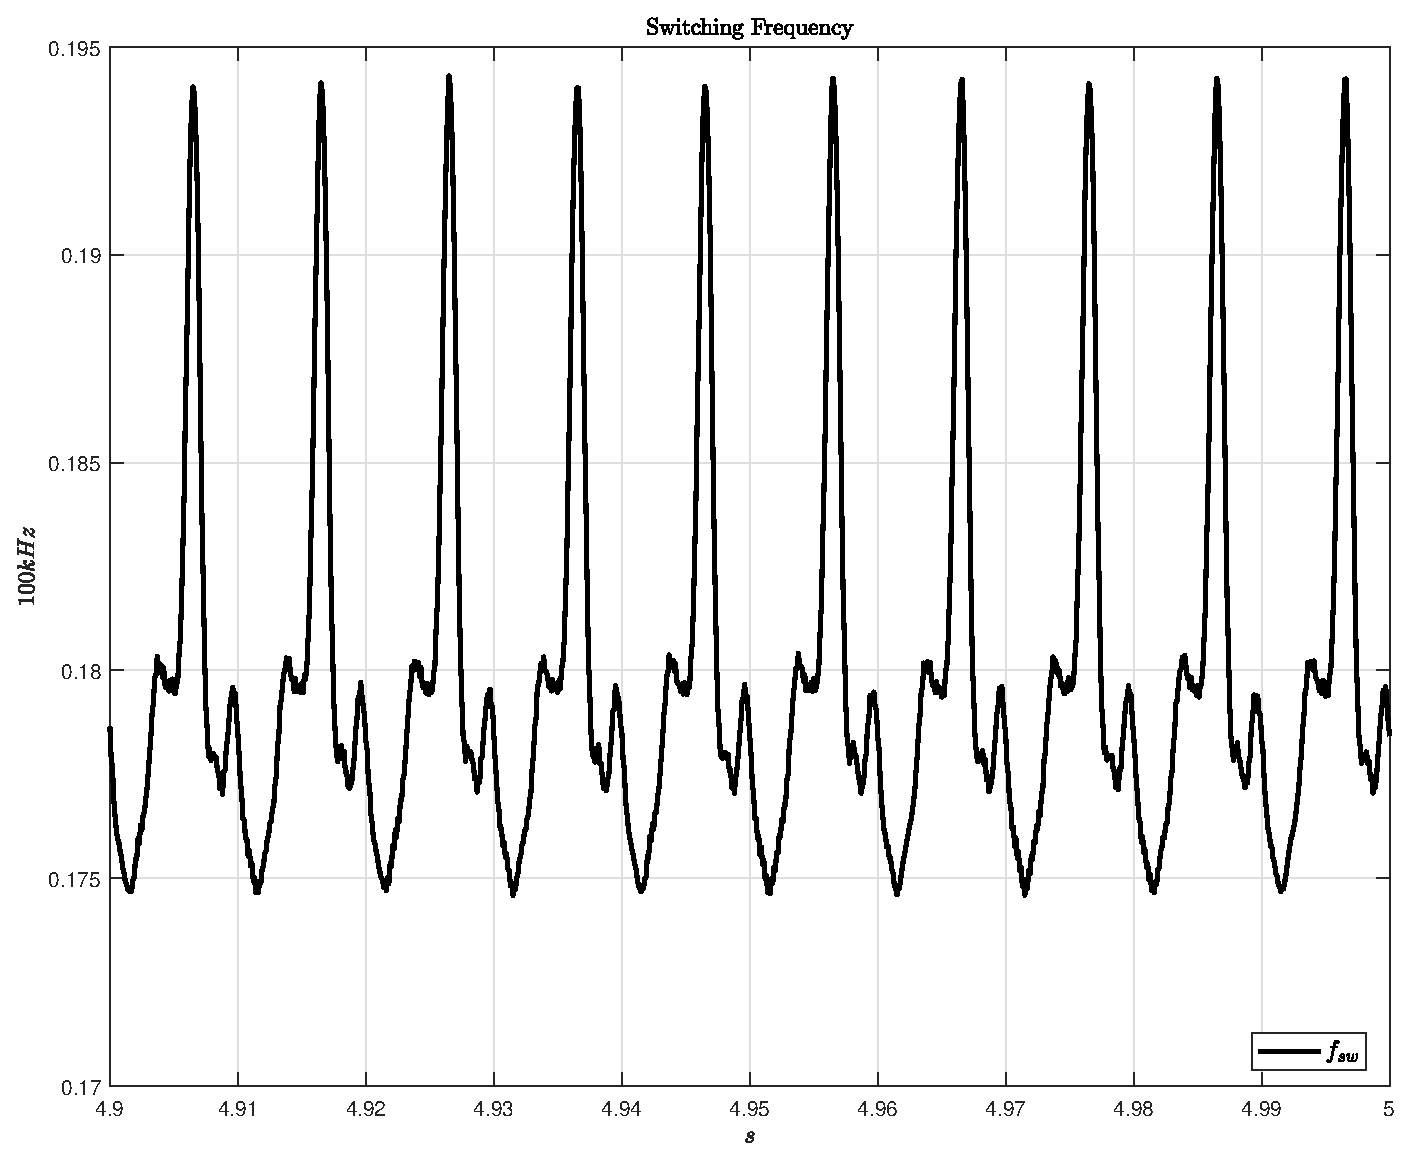
\includegraphics[width = 215pt, angle = 0, 
		keepaspectratio]{figures/sr_with_full_load_3/with_comp_fig_5.eps}
		\captionsetup{width=0.65\textwidth, font=footnotesize}	
		\caption{Control output (frequency switching).}
		\label{}
	\end{subfigure}
	\captionsetup{width=0.5\textwidth, font=small}	
	\caption{Simulation results - case study 6.}
	\label{}
\end{figure}

\chapter{Phase Locked-Loop (PLL) Architecture}
\section{Three-Phase Systems under Unbalanced Conditions}
Three-phases voltages can become unbalanced and distorted because of the effect of nonlinear loads and transient grid faults. Ideally, power converters used in distributed generation should be properly synchronized with the grid under such adverse operating conditions to stay actively connected, supporting the grid services and keeping up generation. The faulty three-phase voltages can be generally understood as a summation of unbalanced harmonic components. Therefore, in general way, the three-phase voltage vector can be written as
\begin{flalign}\label{pll_eq_1}
	\boldsymbol{v}_{rst}=\begin{bmatrix} v_r \\ v_s \\ v_t\end{bmatrix}=\sum_{n=1}^{\infty}\big(\boldsymbol{v}_{rst}^{+n}+\boldsymbol{v}_{rst}^{-n}+\boldsymbol{v}_{rst}^{0n}\big)
\end{flalign}  
where
\begin{flalign}\label{pll_eq_2}
	\boldsymbol{v}_{rst}^{+n} = V^{+n}\begin{bmatrix} 
		\cos\big(n\omega t+\phi^{+n}\big) \\
		\cos\big(n\omega t-\frac{2\pi}{3}+\phi^{+n}\big) \\
		\cos\big(n\omega t+\frac{2\pi}{3}+\phi^{+n}\big)
	\end{bmatrix}
\end{flalign}  
\begin{flalign}\label{pll_eq_3}
	\boldsymbol{v}_{rst}^{-n} = V^{-n}\begin{bmatrix} 
		\cos\big(n\omega t+\phi^{-n}\big) \\
		\cos\big(n\omega t+\frac{2\pi}{3}+\phi^{-n}\big) \\
		\cos\big(n\omega t-\frac{2\pi}{3}+\phi^{-n}\big)
	\end{bmatrix}
\end{flalign}  
\begin{flalign}\label{pll_eq_4}
	\boldsymbol{v}_{rst}^{0n} = V^{0n}\begin{bmatrix} 
		\cos\big(n\omega t+\phi^{0n}\big) \\
		\cos\big(n\omega t+\phi^{0n}\big) \\
		\cos\big(n\omega t+\phi^{0n}\big)
	\end{bmatrix}
\end{flalign}  
In equations \eqref{pll_eq_1}~--~\eqref{pll_eq_4}, superscripts $+n$, $-n$, and $0n$ respectively represent the positive-, negative-, and zero-sequence components of the \textit{n}th harmonic of the voltage vector $\boldsymbol{v}$.

Distributed generators are usually linked to three-phase networks by using a three-wire connection and hence they do not inject zero-sequence current into the grid. 

The main task, for the grid synchronization here investigated, is to find a method to detect and extract the positive sequence component at the fundamental frequency of the three-phase grid voltages.

In a general form, a positive-sequence voltage vector at the fundamental frequency interacting with either a positive- or negative-sequence \textit{n}th order component can be expressed as follows
\begin{flalign}\label{pll_eq_5}
	\boldsymbol{v}_{rst} = \boldsymbol{v}_{rst}^{+1}+\boldsymbol{v}_{rst}^{n}=V^{+1}\begin{bmatrix} 
		\cos\big(\omega t\big) \\[6pt]
		\cos\big(\omega t-\frac{2\pi}{3}\big) \\[6pt]
		\cos\big(\omega t+\frac{2\pi}{3}\big)
	\end{bmatrix}+V^{n}\begin{bmatrix} 
	\cos\big(n\omega t\big) \\[6pt]
	\cos\big(n\omega t-\frac{2\pi}{3}\big) \\[6pt]
	\cos\big(n\omega t+\frac{2\pi}{3}\big)
\end{bmatrix}
\end{flalign}
where $n>0$ means a positive sequence component and $n<0$ a negative sequence one. 

The voltage vector \eqref{pll_eq_5} can be expressed on the Cartesian $\alpha\beta$ stationary reference frame by using a reduced version of the \textit{Clarke} transformation, resulting in
\begin{flalign}\label{pll_eq_6}
	\boldsymbol{v}_{\alpha\beta} = \begin{bmatrix} v_\alpha \\ v_\beta
	\end{bmatrix} = {^{rst}}\mathbf{T}_{\alpha\beta}\boldsymbol{v}_{rst} = V^{+1}\begin{bmatrix}
	\cos\big(\omega t\big) \\[6pt] \sin\big(\omega t\big) \end{bmatrix} + V^{n}\begin{bmatrix}
	\cos\big(n\omega t\big) \\[6pt] \sin\big(n\omega t\big) \end{bmatrix}
\end{flalign}
where 
\begin{flalign}\label{pll_eq_7}
	{^{rst}}\mathbf{T}_{\alpha\beta} = \frac{2}{3}\begin{bmatrix}
		1 & -\frac{1}{2} & -\frac{1}{2} \\[6pt] 0 & \frac{\sqrt{3}}{2} & -\frac{\sqrt{3}}{2}
	\end{bmatrix}
\end{flalign}
The voltage vector \eqref{pll_eq_5} can also be expressed on a Cartesian $dq$ rotating reference frame by using the \textit{Park} transformation as
\begin{flalign}\label{pll_eq_8}
	\boldsymbol{v}_{dq}=\begin{bmatrix}	v_d \\ v_q \end{bmatrix} = {^{\alpha\beta}}\mathbf{T}_{dq} \boldsymbol{v}_{\alpha\beta}= V^{+1}\begin{bmatrix}
		\cos\big(\omega t -\vartheta_{0}\big) \\[6pt] \sin\big(\omega t-\vartheta_{0}\big) \end{bmatrix} + V^{n}\begin{bmatrix}
		\cos\big(n\omega t -\vartheta_{0}\big) \\[6pt] \sin\big(n\omega t-\vartheta_{0}\big) \end{bmatrix}
\end{flalign}
where
\begin{flalign}\label{pll_eq_9}
	{^{\alpha\beta}}\mathbf{T}_{dq} = \begin{bmatrix} \cos\vartheta_{0} & \sin\vartheta_{0} \\[6pt]
		-\sin\vartheta_{0} & \cos\vartheta_{0}
	\end{bmatrix}
\end{flalign}
where $\vartheta_{0}$ is the angular position of the $dq$ rotating reference frame.

Assuming that the $dq$ reference frame rotates synchronously with the positive-sequence voltage vector, with $d$-axis in the same direction as the positive-sequence voltage vector $\boldsymbol{v}^{+1}$, i.e. with $\vartheta_{0}=\omega t$, the expression of \eqref{pll_eq_8} results as follows
 \begin{flalign}\label{pll_eq_10}
 	\boldsymbol{v}_{dq}=V^{+1}\begin{bmatrix} 1 \\ 0 \end{bmatrix} + V^{n}\begin{bmatrix}
 		\cos\big[(n-1)\omega t\big] \\[6pt] \sin\big[(n-1)\omega t\big] \end{bmatrix}
 \end{flalign}
From Eq.~\eqref{pll_eq_10}, the module and the angular position of the three-phase voltage vector, $|\boldsymbol{v}|$ and $\vartheta$ respectively are given by
 \begin{flalign}\label{pll_eq_11}
	|\boldsymbol{v}|=\sqrt{v_{\alpha}^2+v_{\beta}^2} = \sqrt{\big(V^{+1}\big)^2+\big(V^{n}\big)^2+2V^{+1}V^{n}\cos\big[(n-1)\omega t\big]}
\end{flalign}
 \begin{flalign}\label{pll_eq_12}
	\vartheta=\tan^{-1}\frac{v_\beta}{v_\alpha} = \omega t + \tan^{-1}\Big[\frac{V^{n}\sin\big[(n-1)\omega t\big]}{V^{+}+V^{n}\cos\big[(n-1)\omega t\big]}\Big]
\end{flalign}
Equations \eqref{pll_eq_11} and \eqref{pll_eq_12} shows that the voltage vector $\boldsymbol{v}$ has neither constant module nor rotational frequency. Moreover, these equations show that both the amplitude and the angular position of the positive-sequence component cannot be extracted by just filtering the detected module and phase angle of the compound voltage vector $\boldsymbol{v}$.

\section{Synchronous Reference Frame PLL (SRF-PLL)} 
the most extended technique used for frequency-insensitive grid synchronization in the three-phase systems is the PLL based on the synchronous reference frame. The conventional SRF-PLL translates the three-phase voltage vector from the $uvw$ fixed reference frame to the rotating $dq$ reference frame by using \textit{Park}'s transformation $\mathbf{T}_\vartheta$, as shown in Figure~\ref{srf_pll_1}. The angular position of this $dq$ reference frame is controlled by a feedback loop that regulates the $q$ component to zero. Eqs.~\eqref{pll_eq_13}~--~\eqref{pll_eq_15} show the main structure of the transformation from fixed reference frame to the synchronous ($\vartheta$) rotating reference frame.  
 \begin{figure}[H]
 	\centering
 	\includegraphics[width = 400pt, angle = 0, 
 	keepaspectratio]{figures/pll/srf_pll_1.eps}
 	\captionsetup{width=0.5\textwidth, font=small}	
 	\caption{SRF PLL architecture.}
 	\label{srf_pll_1}
 \end{figure}
\begin{flalign}\label{pll_eq_13}
	\begin{bmatrix} v_d \\ v_q \end{bmatrix} = \mathbf{T}_\vartheta\begin{bmatrix} v_r \\ v_s \\ v_t \end{bmatrix}
\end{flalign}
where 
\begin{flalign}\label{pll_eq_14}
	\mathbf{T}_\vartheta = \frac{2}{3}\begin{bmatrix} \cos(\vartheta) & \cos(\vartheta-\frac{2\pi}{3}) & \cos(\vartheta+\frac{2\pi}{3}) \\[6pt] -\sin(\vartheta) & -\sin(\vartheta-\frac{2\pi}{3}) & -\sin(\vartheta+\frac{2\pi}{3}) \end{bmatrix}
\end{flalign}
\begin{flalign}\label{pll_eq_15}
	\mathbf{T}_\vartheta = {^{\alpha\beta}\mathbf{T}_{dq}}{^{rst}\mathbf{T}_{\alpha\beta}}
\end{flalign}
where
\begin{flalign}\label{pll_eq_16}
	{^{rst}\mathbf{T}_{\alpha\beta}} = \frac{2}{3}\begin{bmatrix} 1 & -\frac{1}{2} & -\frac{1}{2} \\[6pt]
		0 & \frac{\sqrt{3}}{2} & -\frac{\sqrt{3}}{2} \end{bmatrix}
\end{flalign}
and 
\begin{flalign}\label{pll_eq_17}
	 {^{\alpha\beta}\mathbf{T}_{dq}}=\begin{bmatrix} \cos\vartheta & \sin\vartheta \\[6pt] -\sin\vartheta & \cos\vartheta \end{bmatrix}
\end{flalign}


\section{Decoupled Double Synchronous Reference Frame PLL (DDSRF-PLL)} 
This section presents an improved three-phase synchronous PLL based on using two synchronous reference frames, rotating with positive and negative synchronous speed, respectively. The usage of this double synchronous reference frame allows decoupling of the effect ot the negative-sequence voltage component on the $dq$ signals detected by the synchronous reference frame rotating with positive angular speed, and vice versa, which makes possible accurate grid synchronization even under unbalanced grid faults.

\subsection{Double synchronous reference frame} 
Figure~\ref{dsrf_1} shows the positive- and negative-sequence components of the unbalanced voltage vector together with a double synchronous reference frame (DSRF) consisting of two rotating reference frame: $dq^{+1}$, rotating with the positive speed $\omega$ and whose angular position is $\vartheta$, and  $dq^{-1}$, rotating with the negative speed $-\omega$ and whose angular position is $-\vartheta$.
\begin{figure}[H]
	\centering
	\includegraphics[width = 250pt, angle = 0, 
	keepaspectratio]{figures/pll/dsrf_1.eps}
	\captionsetup{width=0.5\textwidth, font=small}	
	\caption{Voltage vector and axes of the DSRF.}
	\label{dsrf_1}
\end{figure}
If it is assumed that the angular position reference frame $dq^{+1}$ matches the angular position of the positive-sequence voltage vector $\boldsymbol{v}^{+1}$, i.e. if $\vartheta=\omega t$, the unbalanced input voltage vector $\boldsymbol{v}$ can be expressed on the DSRF, yielding
\begin{flalign}\label{pll_eq_18}
	\boldsymbol{v}_{dq}^{+1} = \begin{bmatrix} v_d^{+1} \\ v_q^{+1}	\end{bmatrix} = \mathbf{T}_{dq}^{+1}\boldsymbol{v}_{\alpha\beta}=V^{+1}\begin{bmatrix} 1 \\ 0 \end{bmatrix}+V^{-1}\begin{bmatrix} \cos(-2\omega t) \\ \sin(-2\omega t) \end{bmatrix}
\end{flalign}
\begin{flalign}\label{pll_eq_19}
	\boldsymbol{v}_{dq}^{-1} = \begin{bmatrix} v_d^{-1} \\ v_q^{-1}	\end{bmatrix} = \mathbf{T}_{dq}^{-1}\boldsymbol{v}_{\alpha\beta}=V^{+1}\begin{bmatrix} \cos(2\omega t) \\ \sin(2\omega t) \end{bmatrix} + V^{-1}\begin{bmatrix} 1 \\ 0 \end{bmatrix}
\end{flalign}
where
\begin{flalign}\label{pll_eq_20}
	\mathbf{T}_{dq}^{+1} = \Big[\mathbf{T}_{dq}^{-1}\Big]^T=\begin{bmatrix} \cos\vartheta & \sin\vartheta \\ -\sin\vartheta & \cos\vartheta
	\end{bmatrix}
\end{flalign}
Expression \eqref{pll_eq_18} and \eqref{pll_eq_19} are evidence that the DC values on the ${dq}^{+1}$ and the ${dq}^{-1}$ frames correspond to the amplitude of the sinusoidal signals of $\boldsymbol{v}^{+1}$ and $\boldsymbol{v}^{-1}$, while the oscillations at $2\omega$ correspond to the coupling between axes appearing as a consequence of the voltage vectors rotating in opposite directions. Therefore, instead of using any filtering techniques for attenuating oscillation at $2\omega$, a decoupling network is presented in the following to completely cancel out the effect of such oscillations on the synchronous reference frame voltages of the PLL.

\subsection{Decoupling network} 
To generalize the explanation of the decoupling network used in the DSRF, one suppose a voltage vector consisting of two components rotating with $n\omega$ and $m\omega$ frequencies respectively, $n$ and $m$ can be either positive or negative. Therefore, this generic voltage vector is given by
\begin{flalign}\label{pll_eq_21}
	\boldsymbol{v}_{\alpha\beta} = \begin{bmatrix} v_\alpha \\[6pt] v_\beta \end{bmatrix} = \boldsymbol{v}_{\alpha\beta}^n + \boldsymbol{v}_{\alpha\beta}^m = V^n\begin{bmatrix} \cos(n\omega t + \phi^n) \\[6pt] \sin(n\omega t + \phi^n) \end{bmatrix} + V^m\begin{bmatrix} \cos(m\omega t + \phi^m) \\[6pt] \sin(m\omega t + \phi^m) \end{bmatrix}
\end{flalign}
Additionally, two rotating reference frames are considered, $dq^n$ and $dq^m$, whose angular positions are $n\vartheta$ and $m\vartheta$ respectively, where $\vartheta$ is the phase angle detected by the PLL. If a perfect synchronization of the PLL is possible, i.e. if $\vartheta = \omega t$, with $\omega$ the fundamental frequency, the voltage vector in \eqref{pll_eq_21} can be expressed on the $dq^n$ and $dq^m$ reference frames as follows
\begin{equation}\label{pll_eq_22}
	\begin{aligned}
		\boldsymbol{v}_{dq}^n&=\begin{bmatrix} v_d^n \\[6pt] v_q^n \end{bmatrix}=\begin{bmatrix} \bar{v}_d^n \\[6pt] \bar{v}_q^n 	\end{bmatrix}+\begin{bmatrix} \tilde{v}_d^n \\[6pt] \tilde{v}_q^n \end{bmatrix} = \underbrace{V^n\begin{bmatrix} \cos\phi^n \\[6pt] \sin\phi^n \end{bmatrix}}_{\text{DC terms}} \\[6pt]
		&+ \underbrace{V^m\cos\phi^m\begin{bmatrix} \cos\big((n-m)\omega t\big) \\[6pt] -\sin\big((n-m)\omega t\big) \end{bmatrix} + V^m\sin\phi^m\begin{bmatrix} \sin\big((n-m)\omega t\big) \\[6pt] \cos\big((n-m)\omega t\big) \end{bmatrix}}_{\text{AC terms}}
	\end{aligned}
\end{equation}
\begin{equation}\label{pll_eq_23}
	\begin{aligned}
		\boldsymbol{v}_{dq}^m &= \begin{bmatrix} v_d^m \\[6pt] v_q^m \end{bmatrix}=\begin{bmatrix} \bar{v}_d^m \\[6pt] \bar{v}_q^m 	\end{bmatrix} +\begin{bmatrix} \tilde{v}_d^m \\[6pt] \tilde{v}_q^m \end{bmatrix} = \underbrace{V^m\begin{bmatrix} \cos\phi^m \\[6pt] \sin\phi^m \end{bmatrix}}_{\text{DC terms}} \\[6pt]
		&+ \underbrace{V^n\cos\phi^n\begin{bmatrix} \cos\big((n-m)\omega t\big) \\[6pt] \sin\big((n-m)\omega t\big) \end{bmatrix} + V^n\sin\phi^n\begin{bmatrix} -\sin\big((n-m)\omega t\big) \\[6pt] \cos\big((n-m)\omega t\big) \end{bmatrix}}_{\text{AC terms}}
	\end{aligned}
\end{equation}
As shown by \eqref{pll_eq_22}~and~\eqref{pll_eq_23}, the amplitude of the AC terms in the $dq^n$ axes depends on the DC terms of the signals on the $dq^m$ axes, and vice versa. Therefore, once the coupling terms between both reference frames are identified, a decoupling cell, can be designed to cancel out the oscillations generated by the voltage vector $\boldsymbol{v}^m$ on the $dq^n$ axes signals. To cancel out the oscillations in the $dq^m$ axes signals, the same structure may be used, but with swapping of the $m$ and $n$ indexes in it. In Figure~\ref{decoupling_cell_1}, the DC terms on the $dq^n$ axes are represented as $\bar{v}_d^m$ and $\bar{v}_q^m$.

As shown in Figure~\ref{ddsrf_pll_2}, a cross-feedback decoupling network is used to estimate the value of these DC terms on the positive and negative reference frames. In this decoupling network, the estimated DC terms are named as $(\bar{v}_d^m)^*$, $(\bar{v}_q^m)^*$, $(\bar{v}_d^n)^*$ and $(\bar{v}_q^n)^*$ and LPF block is a low pass filter such as
\begin{flalign}\label{pll_eq_24}
	LPF(s) = \frac{\omega_{f}}{s+\omega_{f}}
\end{flalign}
\begin{figure}[H]
	\centering
	\includegraphics[width = 325pt, angle = 0, 
	keepaspectratio]{figures/pll/decoupling_cell_1.eps}
	\captionsetup{width=0.5\textwidth, font=small}	
	\caption{Decoupling cell for cancelling the effect of $\boldsymbol{v}^m$ on the $dq^n$ frame signals.}
	\label{decoupling_cell_1}
\end{figure}
The decoupled double synchronous reference frame (DDSRF) of Figure~\ref{ddsrf_pll_2} allows free-oscillation signals to be obtained on the $dq^m$ and $dq^n$ reference frame. By setting $n=+1$ and $m=-1$, this network decouples information about the positive and negative sequence components of either voltage or current in unbalanced three-phase systems, which makes it a useful tool for synchronous controllers during unbalanced grid faults. This network can be used to decouple other frequency/sequence components simply setting the proper values for the $m$ and $n$ coefficients.
\begin{figure}[H]
	\centering
	\includegraphics[width = 450pt, angle = 0, 
	keepaspectratio]{figures/pll/ddsrf_pll_2.eps}
	\captionsetup{width=0.5\textwidth, font=small}	
	\caption{Decoupled double synchronous reference frame (DDSRF).}
	\label{ddsrf_pll_2}
\end{figure}
\subsection{Analysis of the DDSRF} 
From Eq.~\eqref{pll_eq_21}, the unbalanced voltage during a grid fault, consisting of positive- and negative-sequence components at the fundamental frequency, can be generically expressed as 
\begin{flalign}\label{pll_eq_25}
	\boldsymbol{v}_{\alpha\beta} = \begin{bmatrix} v_\alpha \\[6pt] v_\beta \end{bmatrix} = \boldsymbol{v}_{\alpha\beta}^{+1} + \boldsymbol{v}_{\alpha\beta}^{-1} = V^{+1}\begin{bmatrix} \cos(\omega t + \phi^{+1}) \\[6pt] \sin(\omega t + \phi^{+1}) \end{bmatrix} + V^{-1}\begin{bmatrix} \cos(-\omega t + \phi^{-1}) \\[6pt] \sin(-\omega t + \phi^{-1}) \end{bmatrix}
\end{flalign}
The projection of this voltage vector on the $dq^{+1}$ and $dq^{-1}$ reference frames can be easily obtained simply by setting $n=+1$ and $m=-1$ in \eqref{pll_eq_22} and \eqref{pll_eq_23}. After rearranging equations, the $dq$ signals on the positive and negative reference frames are given by
\begin{flalign}
		\boldsymbol{v}_{dq}^{+1} &= {V^{+1}\begin{bmatrix} \cos\phi^{+1} \\[6pt] \sin\phi^{+1} \end{bmatrix}} + V^{-1}\begin{bmatrix} \cos\big(2\omega t\big) & \sin\big(2\omega t\big) \\[6pt] -\sin\big(2\omega t\big) & \cos\big(2\omega t\big) \end{bmatrix} \begin{bmatrix} \cos\phi^{-1} \\[6pt] \sin\phi^{-1} \end{bmatrix} \label{pll_eq_26} \\[6pt]
		\boldsymbol{v}_{dq}^{-1} &= {V^{-1}\begin{bmatrix} \cos\phi^{-1} \\[6pt] \sin\phi^{-1} \end{bmatrix}} + V^{+1}\begin{bmatrix} \cos\big(2\omega t\big) & -\sin\big(2\omega t\big) \\[6pt] \sin\big(2\omega t\big) & \cos\big(2\omega t\big) \end{bmatrix} \begin{bmatrix} \cos\phi^{+1} \\[6pt] \sin\phi^{+1} \end{bmatrix} \label{pll_eq_27}
\end{flalign}
 These expressions give evidence that the AC terms in the $dq^{+1}$ axes result from the DC terms in the $dq^{-1}$ axes being affected by a rotating transformation matrix at $2\omega$ frequency. A similar conclusion can be obtained for AC signals of the $dq^{-1}$ reference frame. These rotating transformation matrices are given b y
 \begin{flalign}\label{pll_eq_28}
 	\mathbf{T}_{dq}^{+2} = \Big(\mathbf{T}_{dq}^{-2}\Big)^T = \begin{bmatrix} \cos(2\omega t)  &  \sin(2\omega t) \\[6pt] -\sin(2 \omega t) & \cos(2 \omega t\end{bmatrix}
 \end{flalign}
Therefore Eqs,~\eqref{pll_eq_26}~--~\eqref{pll_eq_27} can be rewritten as follows 
\begin{flalign}
	\boldsymbol{v}_{dq}^{+1} &= \begin{bmatrix} v_d^{+1} \\[6pt] v_q^{+1} \end{bmatrix} = \bar{\boldsymbol{v}}_{dq}^{+1} + \mathbf{T}_{dq}^{+2} \bar{\boldsymbol{v}}_{dq}^{-1} \label{pll_eq_29} \\[6pt]
	\boldsymbol{v}_{dq}^{-1} &= \begin{bmatrix} v_d^{-1} \\[6pt] v_q^{-1} \end{bmatrix} = \bar{\boldsymbol{v}}_{dq}^{-1} + \mathbf{T}_{dq}^{-2} \bar{\boldsymbol{v}}_{dq}^{+1} \label{pll_eq_30}
\end{flalign}
where 
\begin{flalign}
	\bar{\boldsymbol{v}}_{dq}^{+1} &= \begin{bmatrix} \bar{v}_d^{+1} \\[6pt] \bar{v}_q^{+1} \end{bmatrix} = V^{+1}\begin{bmatrix} \cos\phi^{+1} \\[6pt] \sin\phi^{+1} \end{bmatrix} \label{pll_eq_31}
\end{flalign}
and
\begin{flalign}
	\bar{\boldsymbol{v}}_{dq}^{-1} &= \begin{bmatrix} \bar{v}_d^{-1} \\[6pt] \bar{v}_q^{-1} \end{bmatrix} = V^{-1}\begin{bmatrix} \cos\phi^{-1} \\[6pt] \sin\phi^{-1} \end{bmatrix} \label{pll_eq_32}
\end{flalign}
represent the amplitude of the sequence components applied to the input of the DDSRF. Thus, Eqs.~\eqref{pll_eq_29}~--~\eqref{pll_eq_30} give evidence that the relationship between the signals on the positive and negative reference frames are given by
\begin{flalign}
	\boldsymbol{v}_{dq}^{+1} &= \mathbf{T}_{dq}^{+2} \boldsymbol{v}_{dq}^{-1} \label{pll_eq_33} 
\end{flalign}
and 
\begin{flalign}
	\boldsymbol{v}_{dq}^{-1} &= \mathbf{T}_{dq}^{-2} \boldsymbol{v}_{dq}^{+1} \label{pll_eq_34} 
\end{flalign}
As a result, the estimated values of the output of the DDSRF can be written as follows
\begin{flalign}
	\big(\bar{\boldsymbol{v}}_{dq}^{+1}\big)^* &= \begin{bmatrix}
		\big(\bar{{v}}_{d}^{+1}\big)^* \\[6pt] \big(\bar{{v}}_{q}^{+1}\big)^* \end{bmatrix} = \mathbf{F}(s) \Big[\boldsymbol{v}_{dq}^{+1} -\mathbf{T}_{dq}^{+2} \big(\bar{\boldsymbol{v}}_{dq}^{-1}\big)^*\Big] \label{pll_eq_35} \\[6pt] 
	\big(\bar{\boldsymbol{v}}_{dq}^{-1}\big)^* &= \begin{bmatrix}
		\big(\bar{{v}}_{d}^{-1}\big)^* \\[6pt] \big(\bar{{v}}_{q}^{-1}\big)^* \end{bmatrix} = \mathbf{F}(s) \Big[\boldsymbol{v}_{dq}^{-1} -\mathbf{T}_{dq}^{-2} \big(\bar{\boldsymbol{v}}_{dq}^{+1}\big)^*\Big] \label{pll_eq_36}
\end{flalign}
where 
\begin{flalign} \label{pll_eq_37}
	\mathbf{F}(s) = \begin{bmatrix} LPF(s) & 0 \\[6pt] 0 & LPF(s) \end{bmatrix}
\end{flalign}
\begin{figure}[H]
	\centering
	\includegraphics[width = 350pt, angle = 0, 
	keepaspectratio]{figures/pll/ddsrf_pll_3.eps}
	\captionsetup{width=0.5\textwidth, font=small}	
	\caption{Block diagram of the DDSRF with $n=+1$ and $m=-1$.}
	\label{ddsrf_pll_3}
\end{figure}
Therefore, the DDSRF of Figure~\ref{ddsrf_pll_2} can be represented for the particular case of the positive- and negative-sequence components at the fundamental frequency, as in Figure~\ref{ddsrf_pll_3} shows. The estimation of the positive sequence component will be considered in the following. Substituting \eqref{pll_eq_36} into \eqref{pll_eq_35} it results
\begin{flalign} \label{pll_eq_37}
	\big(\bar{\boldsymbol{v}}_{dq}^{+1}\big)^* &= \mathbf{F}(s)\Bigg[\boldsymbol{v}_{dq}^{+1}-\mathbf{T}_{dq}^{+2} \mathbf{F}(s)\Big(\boldsymbol{v}_{dq}^{-1} -\mathbf{T}_{dq}^{-2} \big(\bar{\boldsymbol{v}}_{dq}^{+1}\big)^*\Big)\Bigg]
\end{flalign}
and using the relationship of \eqref{pll_eq_33} and \eqref{pll_eq_34}, it results
\begin{flalign} \label{pll_eq_38}
	\big(\bar{\boldsymbol{v}}_{dq}^{+1}\big)^* &= \mathbf{F}(s)\Bigg[\boldsymbol{v}_{dq}^{+1}-\mathbf{T}_{dq}^{+2} \mathbf{F}(s)\Big(\mathbf{T}_{dq}^{-2} \boldsymbol{v}_{dq}^{+1} -\mathbf{T}_{dq}^{-2} \big(\bar{\boldsymbol{v}}_{dq}^{+1}\big)^*\Big)\Bigg]
\end{flalign}
rearranging, it results
\begin{flalign} \label{pll_eq_39}
	\big(\bar{\boldsymbol{v}}_{dq}^{+1}\big)^* &= \mathbf{F}(s)\Bigg[\boldsymbol{v}_{dq}^{+1}-\mathbf{T}_{dq}^{+2} \mathbf{F}(s)\mathbf{T}_{dq}^{-2}\Big(\boldsymbol{v}_{dq}^{+1} -\big(\bar{\boldsymbol{v}}_{dq}^{+1}\big)^*\Big)\Bigg]
\end{flalign}
The term $\mathbf{T}_{dq}^{+2} \mathbf{F}(s)\mathbf{T}_{dq}^{-2}$ will be now investigated
\begin{equation} \label{pll_eq_40}
	\begin{aligned}
		\mathbf{F}_{-2}(s) &= \mathbf{T}_{dq}^{+2} \mathbf{F}(s)\mathbf{T}_{dq}^{-2} \\[6pt]
		&=\frac{1}{2} \begin{bmatrix} 
			\big[\mathbf{F}(s+j2\omega)+\mathbf{F}(s-j2\omega)\big] & j\big[-\mathbf{F}(s+j2\omega)+\mathbf{F}(s-j2\omega)\big] \\[6pt]
			j\big[\mathbf{F}(s+j2\omega)+\mathbf{F}(s-j2\omega)\big] & \big[\mathbf{F}(s+j2\omega)+\mathbf{F}(s-j2\omega)\big] 
		\end{bmatrix}
	\end{aligned}
\end{equation}
which results as follows
\begin{equation} \label{pll_eq_41}
	\begin{aligned}
		\mathbf{F}_{-2}(s) = \mathbf{F}_{+2}^T(s) = \frac{1}{2}\begin{bmatrix} \frac{\omega_{f}(s+\omega_{f})}{s^2+2s\omega_{f}+\omega_{f}^2+(2\omega)^2} & -\frac{\omega_{f}\omega}{s^2+2s\omega_{f}+\omega_{f}^2+(2\omega)^2} \\[8pt] \frac{\omega_{f}\omega}{s^2+2s\omega_{f}+\omega_{f}^2+(2\omega)^2} & \frac{\omega_{f}(s+\omega_{f})}{s^2+2s\omega_{f}+\omega_{f}^2+(2\omega)^2}
		\end{bmatrix}
	\end{aligned}
\end{equation}


\subsection{Structure of the DDSRF-PLL}
The block diagram of the DDSRF-PLL is shown in Figure~\ref{ddsrf_pll_5}. As shown in the figure, this PLL is an extension of the conventional three-phase SRF-PLL structure. In this PLL, in order to obtain a similar dynamic response for different signal amplitudes, the phase-angle error signal $v_q^{+1}$ is adaptively normalized to the amplitude of the positive-sequence input vector. Moreover, the rated grid frequency is added as a feed-forward parameter, $\omega_{ff}$, to accelerate the tracking process of the PLL. The decoupling network of the DDSRF-PLL completely cancels out the oscillations at $2\omega$ on the $d1^{+1}$ and $d1^{-1}$ reference frame signals. 
\begin{figure}[H]
	\centering
	\includegraphics[width = 400pt, angle = 0, 
	keepaspectratio]{figures/pll/ddsrf_pll_5.eps}
	\captionsetup{width=0.5\textwidth, font=small}	
	\caption{DDSRF PLL architecture.}
	\label{ddsrf_pll_5}
\end{figure}
\begin{figure}[H]
	\centering
	\includegraphics[width = 400pt, angle = 0, 
	keepaspectratio]{figures/pll/ddsrf_pll_1.eps}
	\captionsetup{width=0.5\textwidth, font=small}	
	\caption{DDSRF PLL architecture - a different representation.}
	\label{ddsrf_pll_1}
\end{figure}
\section{Simulation Results}
In this section SRF-PLL and DDSRF-PLL performances are compared. Figure~\ref{grid_voltage_srf_pll_fig_1} shows a set of unbalanced grid voltages used as source for both pll architectures.  
\begin{figure}[H]
	\centering
	\includegraphics[width = 225pt, angle = 0, 
	keepaspectratio]{figures/pll/grid_voltage_srf_pll_fig_1.eps}
	\captionsetup{width=0.5\textwidth, font=small}	
	\caption{Grid voltage used for simulation analysis.}
	\label{grid_voltage_srf_pll_fig_1}
\end{figure}
Figure~\ref{grid_phase_srf_pll_fig_2} shows the performance for phase and frequency estimation of the SRF-PLL in case of unbalanced grid voltages. As can be seen, both of them are affected by a second component (\SI{100}{\hertz}) harmonic generated by the fact the grid voltages are unbalanced.
\begin{figure}[H]
	\centering
	\begin{subfigure}{0.5\textwidth}
		\centering
		\includegraphics[width = 225pt, angle = 0, 
		keepaspectratio]{figures/pll/grid_phase_srf_pll_fig_2.eps}
		\captionsetup{width=0.65\textwidth, font=footnotesize}	
		\caption{Phase and pulsation estimated by the SRF-PLL.}
		\label{grid_phase_srf_pll_fig_2}
	\end{subfigure}%
	\begin{subfigure}{0.5\textwidth}
		\centering
		\includegraphics[width = 225pt, angle = 0, 
		keepaspectratio]{figures/pll/grid_phase_ddsrf_pll_fig_2.eps}
		\captionsetup{width=0.65\textwidth, font=footnotesize}	
		\caption{Phase and pulsation estimated by the DDSRF-PLL.}
		\label{grid_phase_ddsrf_pll_fig_2}
	\end{subfigure}
	\captionsetup{width=0.5\textwidth, font=small}	
	\caption{Simulation results.}
	\label{}
\end{figure}
%\begin{figure}[H]
%	\centering
%	\includegraphics[width = 300pt, angle = 0, 
%	keepaspectratio]{figures/pll/grid_phase_srf_pll_fig_2.eps}
%	\captionsetup{width=0.5\textwidth, font=small}	
%	\caption{Phase and pulsation estimated by the SRF-PLL.}
%	\label{grid_phase_srf_pll_fig_2}
%\end{figure}
Figure~\ref{grid_phase_ddsrf_pll_fig_2} shows the performance for phase and frequency estimation of the DDSRF-PLL in case of unbalanced grid voltages. As can be seen, the second harmonic which was present for the SRF-PLL case is completely compensated by the structure of the PLL, and estimated phase as well as estimated grid frequency results not affected by the unbalanced grid voltages. 
%\begin{figure}[H]
%	\centering
%	\includegraphics[width = 300pt, angle = 0, 
%	keepaspectratio]{figures/pll/grid_phase_ddsrf_pll_fig_2.eps}
%	\captionsetup{width=0.5\textwidth, font=small}	
%	\caption{Phase and pulsation estimated by the DDSRF-PLL.}
%	\label{grid_phase_ddsrf_pll_fig_2}
%\end{figure}

\begin{thebibliography}{99}
	% power electronics
	\bibitem{kazimierczuk} 
	M. K. Kazimierczuk, D. Czarkowski, \emph{Resonant Power Converters}. Wiley, 2nd Edition 2011.

	\bibitem{liserre} 
	R. Teodorescu, M. Liserre, P. Rodrıguez, \emph{Grid converters for photovoltaic and wind power systems}. Wiley, 2011.
\end{thebibliography}

\end{onehalfspace}
\end{document} 